\documentclass[12pt, a4paper]{article}
\usepackage[margin=2.0cm]{geometry}
\usepackage[utf8]{inputenc}
\usepackage[document]{ragged2e}
\usepackage{listings}
\pagenumbering{arabic}
\usepackage{xcolor}

%za dodavanje slika i putanje gde se nalaze slike
\usepackage{graphicx}
\usepackage{float}
\graphicspath{ {./missing_values_visual/}{./geolocation_visual/} {./knime/knime_slike/} {./knime/knime_slike/kMeans_childrenKI/} {./knime/knime_slike/dbscan_childrenKI/} {./knn_python/}}

%definisemo boje koje koristimo
\definecolor{mygreen}{rgb}{0,0.6,0}
\definecolor{mygray}{rgb}{0.5,0.5,0.5}
\definecolor{mymauve}{rgb}{0.58,0,0.82}
\definecolor{backcolour}{rgb}{0.9,0.9,0.9}

%specijalni karakter dj
\def\DJ{\leavevmode\setbox0=\hbox{D}\kern0pt
\rlap{\kern.04em\raise.188\ht0\hbox{-}}D}
\def\dj{\leavevmode\setbox0=\hbox{d}\kern0pt
\rlap{\kern.215em\raise.46\ht0\hbox{-}}d}

%setujemo zeljene opcije za blok koda
\lstset{
	language=Python,
	basicstyle=\footnotesize\ttfamily\color{black},
	commentstyle=\color{mygreen},
	morecomment=[l][\color{magenta}]{\#},
  	keywordstyle=\color{blue},
  	stringstyle=\color{mymauve},
	frame=single,
	backgroundcolor=\color{backcolour},
	numbers=left,
	numbersep=5pt,
	numberstyle=\tiny\color{mygray},
	showspaces=false,
	showstringspaces=false,
	tabsize=4,
  	breaklines=true
}

%linkovi
\usepackage{hyperref}
\hypersetup{
    colorlinks=true,
    linkcolor=blue,
    filecolor=magenta,      
    urlcolor=cyan,
}

%naslov i autori
\title{\textbf{Analiza skupa podataka\\ Children Killed or Injured\\}- Seminarski rad - \\Istra\v zivanje podataka \\ Matemati\v cki fakultet}
\author{Zorana Gaji\' c 400/2016 \\ David Dimi\' c 137/2015}
\date{Beograd 2018.}

%preimenovanje
\renewcommand{\contentsname}{Sadr\v zaj}
\renewcommand{\listfigurename}{Slike}
\renewcommand{\figurename}{Slika}
\renewcommand{\listtablename}{Tabele}
\renewcommand{\tablename}{Tabela}

\begin{document}

\begin{titlepage}
\maketitle
\thispagestyle{empty}
\end{titlepage}

\tableofcontents
\clearpage


\section {Uvod}
Istra\v zivanje podataka sastoji iz tri faze:
\begin{itemize}
\item prikupljanje podataka
\item ekstrakcija i \v ci\v s\' cenje podataka
\item analiti\v cka obrada i algoritmi
\end{itemize}

Podaci predstavljaju izve\v staje o nesre\' cama i ubistvima dece u gradovima Amerike. 
\break 
%TODO Pitanja sta sve zelimo istraziti


\section {Prikupljanje podataka}
Podaci su prikupljani sa: \url{http://www.gunviolencearchive.org/reports/}
i to: \begin{list}{•}{}
\item Children Killed
\item Children Injured
\item Accidental Deaths (Children Ages 0-11)
\item Accidental Injuries (Children Ages 0-11)
\end{list}

Ponu\dj eni .csv fajl sadr\v zi premalo atributa, u svakom fajlu po 6 (Incident Date, State, City Or County, Address, Killed, Injured). Dok kada se klikne na View Incident dobije se mnogo vi\v se korisnih podataka za taj konkretan incident. 
\break 

Na\v s cilj je prvo prikupiti te dodatne podatke i od njih formirati nove .csv fajlove sa ne\v sto pogodnijim atributima za rad, a potom te novoprikupljene dalje obra\dj ivati.

Za to je bilo korisno nekoliko linux alatki iz terminala kao i programski jezik \textbf{Python3}.

Za svaku kolonu sa sajta treba skinuti html stranicu do koje se dolazi klikom na View Incident. Po\v sto u svaki fajl ima oko 500 redova to smo ostvarili rekurzivnim obilaskom sajta pomo\' cu alatke \textbf{wget}:

\begin{verbatim}
wget -np -r -R "index.html*" -l 1 "http://www.gunviolencearchive.org/children-killed"
\end{verbatim}
Potrebno je tako\dj e postaviti dubinu rekurzije na 1 (flag -l 1) da se ne bi, ulaze\' ci u druge linkove, krenulo u obilazak celog sajta. Potom je to isto potrebno uraditi za sve stranice, a da se ne bi radilo ru\v cno napravljen je slede\' ci jednostavan python skript:

\begin{lstlisting}
import os

for i in range(2,18):
    os.system("wget -np -r -R \"index.html*\" -l 1  \"http://www.gunviolencearchive.org/children-killed?page=" + str(i) + "\"")
\end{lstlisting}
Po\v sto imamo prikupljene potrebne html strane mo\v zemo pristupiti parsiranju html-a i izdvajanju \v zeljenih atributa. Kori\v s\' ceni su regularni izrazi (modul \textbf{re}) u pythonu.

\break
Jedan primer dela html strane \textit{Incident} sa koje je potrebno izdvojiti \v zeljene podatke:

\begin{verbatim}
Location

    June 12, 2016
    first block of James Avenue
    Littlestown, Pennsylvania
    Geolocation: 39.7448, -77.092

Participants

    -Type: Victim
    -Name: Codie Powell
    -Age: 9
    -Age Group: Child 0-11
    -Gender: Female
    -Status: Killed

    -Type: Victim
    -Name: Talisaha Powell
    -Age Group: Adult 18+
    -Gender: Female
    -Status: Injured

    -Type: Subject-Suspect
    -Relationship: Family
    -Name: Donald Powell
    -Age: 37
    -Age Group: Adult 18+
    -Gender: Male
    -Status: Killed
\end{verbatim}

Odgovaraju\' cim regularnim izrazima mo\v zemo izdvojiti \v zeljene podatke, ali treba ima na umu da redosled podataka nije uniforman na svim stranicama. Na primer, uo\v ceno je da u nekim redosled \textit{Gender} pa \textit{Status}, dok je u drugim njihov redosled zamenjen.
\break
Tako\dj e, u novim tabelama bi\' ce vi\v se redova nego u originalnim jer dodajemo redove za svakog od u\v cesnika, kojih mo\v ze biti vi\v se za jedan isti doga\dj aj. Ba\v s zbog te osobine dodat je novi atribut: \textit{ID} koji je isti za iste doga\dj aje (incidente).
\break

Ilustrujmo male delove python koda koji od odeljka \textit{Participants} formira atribute: Type, Name, Age, Age Group, Gender i Status.
\break

Analizom html-a uo\v cavamo grupaciju koja se odnosi na u\v cesnike i formiramo odgovaraju\' ce regularne izlaze, a potom podatke tra\v zimo unutar tog bloka izdvajanjem cele liste (izme\dj u tagova  $<ul>$. Jedna lista odgovara podacima o jednoj osobi), dok unutar njega grupi\v semo elemente liste (izme\dj u tagova  $<li>$) i to sve levo i desno od znaka dvota\v cke
\footnote{Poslednji regex je napravljen posebno po\v sto se koristi na vi\v se mesta u kodu}:

\newpage
\begin{lstlisting}
#ucesnici
re_participants = re.compile(r"""
     <\s*h2\s*>\s*Participants\s*<\s*\/h2\s*>(.|\s)*?</div
     """, re.VERBOSE)

#ucesnici, suzen izbor
re_regex1 = re.compile(r"""
    <\s*ul\s*>(.|\s)*?<\s*\/ul\s*>
    """, re.VERBOSE)
    
#type:value
re_regex_type_value = re.compile(r"""
    <li\s*>(?P<type>(.|\s)*?):(?P<value>(.|\s)*?)<
    """, re.VERBOSE)
\end{lstlisting}

Dalje se ovako definisani regularni izrazi koriste u kodu:
\begin{lstlisting}
#svi ucesnici
#siri kontekst - trazenje dela sa Participants
x = re_participants.search(html_file)
if x != None:
    participants = x.group()

	#uzi kontekst - trazenje pojedinacnih ucesnika
    for z in re_regex1.finditer(participants):
        subject = z.group()

		#pretpostavimo da sve od navedenog za svaku osobu 
		#moze da nedostaje
		#ako se dokaze suprotno dodelicemo nadjenu vrednost
        Type = "N/A"
        Name = "N/A"
        Age = "N/A"
        Age_group = "N/A"
        Gender = "N/A"
        Status = "N/A"

		#za svakog ucesnika trazimo atribute
		#type, name, age, age group, gender i status
        for y in re_regex_type_value.finditer(subject):
            key = y.group('type').strip()
            value = y.group('value').strip()

            if key == 'Type':
                Type = value
            elif key == 'Name':
                Name = value
            elif key == 'Age':
                Age = value
            elif key == 'Age Group':
                Age_group = value
            elif key == 'Gender':
                Gender = value
            elif key == 'Status':
                Status = value
                
         #upisivanje ucesnika u izlaznu datoteku...

\end{lstlisting}

\newpage
Ovim smo obezbedili da mo\v ze imati vi\v se osoba i da redosled njihov atributa nije bitan. Slu\v caj nedostaju\' cih vrednosti tako\dj e je pokriven. Na sli\v can na\v cin izdvoje se i ostali potrebni podaci, a sve to izvr\v sava se u obilasku prosle\dj enog direktorijuma u kojem se nalaze sve potrebne html stranice, \v sto je mogu\' ce izvesti sa os.walk(path) funkcijom.

\section {Ekstrakcija i \v ci\v s\' cenje podataka}
\subsection {Opis podataka}

Vi\v se redova u tabeli predstavlja informacije o jednom doga\dj aju, s obzirom da u jednom doga\dj aju 
mo\v ze u\v cestvovati vi\v se ljudi, odnosno \v zrtve i osumnji\v ceni.
\break
Na raspolaganju su nam atributi sa tabele:

\begin{table}[H]
\label{table:atributi}
\begin{tabular}{ |p{3cm}||p{3cm}|p{6.5cm}|p{3cm}|  }
 \hline
 \multicolumn{4}{|c|}{Podaci} \\
 \hline
 	Atribut& Tip atributa &Mogu\' ce vrednosti &Nedostaju\' ce vrednosti\\
 \hline
 	ID & Kvantitativni & 0-100000	& NE \\
 	Incident Date& Kategori\v cki & Datum oblika: Month Date, Year & NE \\
 	State& Kategori\v cki& & NE\\
 	City& Kategori\v cki& & NE\\
 	Geolocation& Kvantitativni& Koordinate oblika: double, double & DA\\
 	Guns Involved& Kvantitativni& 1-4& DA\\
 	Gun Types& Kategori\v cki& tipovi oru\v zja& DA\\
 	Guns Stolen& Kategori\v cki, binarni& Not-stolen, Stolen& DA\\
 	Type& Kategori\v cki, binarni & Victim, Subject - Suspect & NE\\
 	Name& Kategori\v cki & First Name, Last Name & DA\\
 	Age& Kvantitativni & 1-82 & DA \\
 	Age Group& Kategori\v cki, binarni & Child 0-11, Adult 18+ & DA\\
 	Gender& Kategori\v cki, binarni & Male, Female & DA \\
 	Status& Kategori\v cki & Arrested, Injured, Injured Arested, Killed, Unharmed, Unharmed Arested & DA \\
 \hline
\end{tabular}
\caption{Atributi i njihove karakteristike}
\end{table}


\break
 

\subsection {Vizualna reprezentacija polaznih podataka}
Da bismo stekli bolji ose\' caj i uvid u to sa kakvim podacima radimo vizualno smo prestavili samo neke interesantne njihove aspekte pre ikakve obrade. Ovim mo\v ze da se stekne bolja slika kojim putem krenuti u obradu i koje algoritme primeniti.

\subsubsection{Nedostaju\' ce vrednosti}
Koriste\' ci python modul \textbf{missingno} reprezentovali smo nedostaju\' ce vrednosti nad slu\v cajnim uzorkom od 250 redova \footnote{Preporuka kori\v s\' cenog modula} za svaku od \v cetiri tabele.

\begin{lstlisting}
import sys
import pandas
import missingno
import matplotlib.pyplot as plt

args = sys.argv
if len(args) != 2:
    sys.exit(f"usage: ./{args[0]} /path/to/.csv")

#ucitavanje iz prosledjenog csv fajla
df = pandas.read_csv(args[1])
#plotovanje missingo rezultata
plt.show(missingno.matrix(df.sample(250)))
\end{lstlisting}

Dobijamo slede\' ce grafikone na kojima se jasno vidi kakva nam je raspodela nedostaju\' cih vrednosti:

\begin{figure}[H]
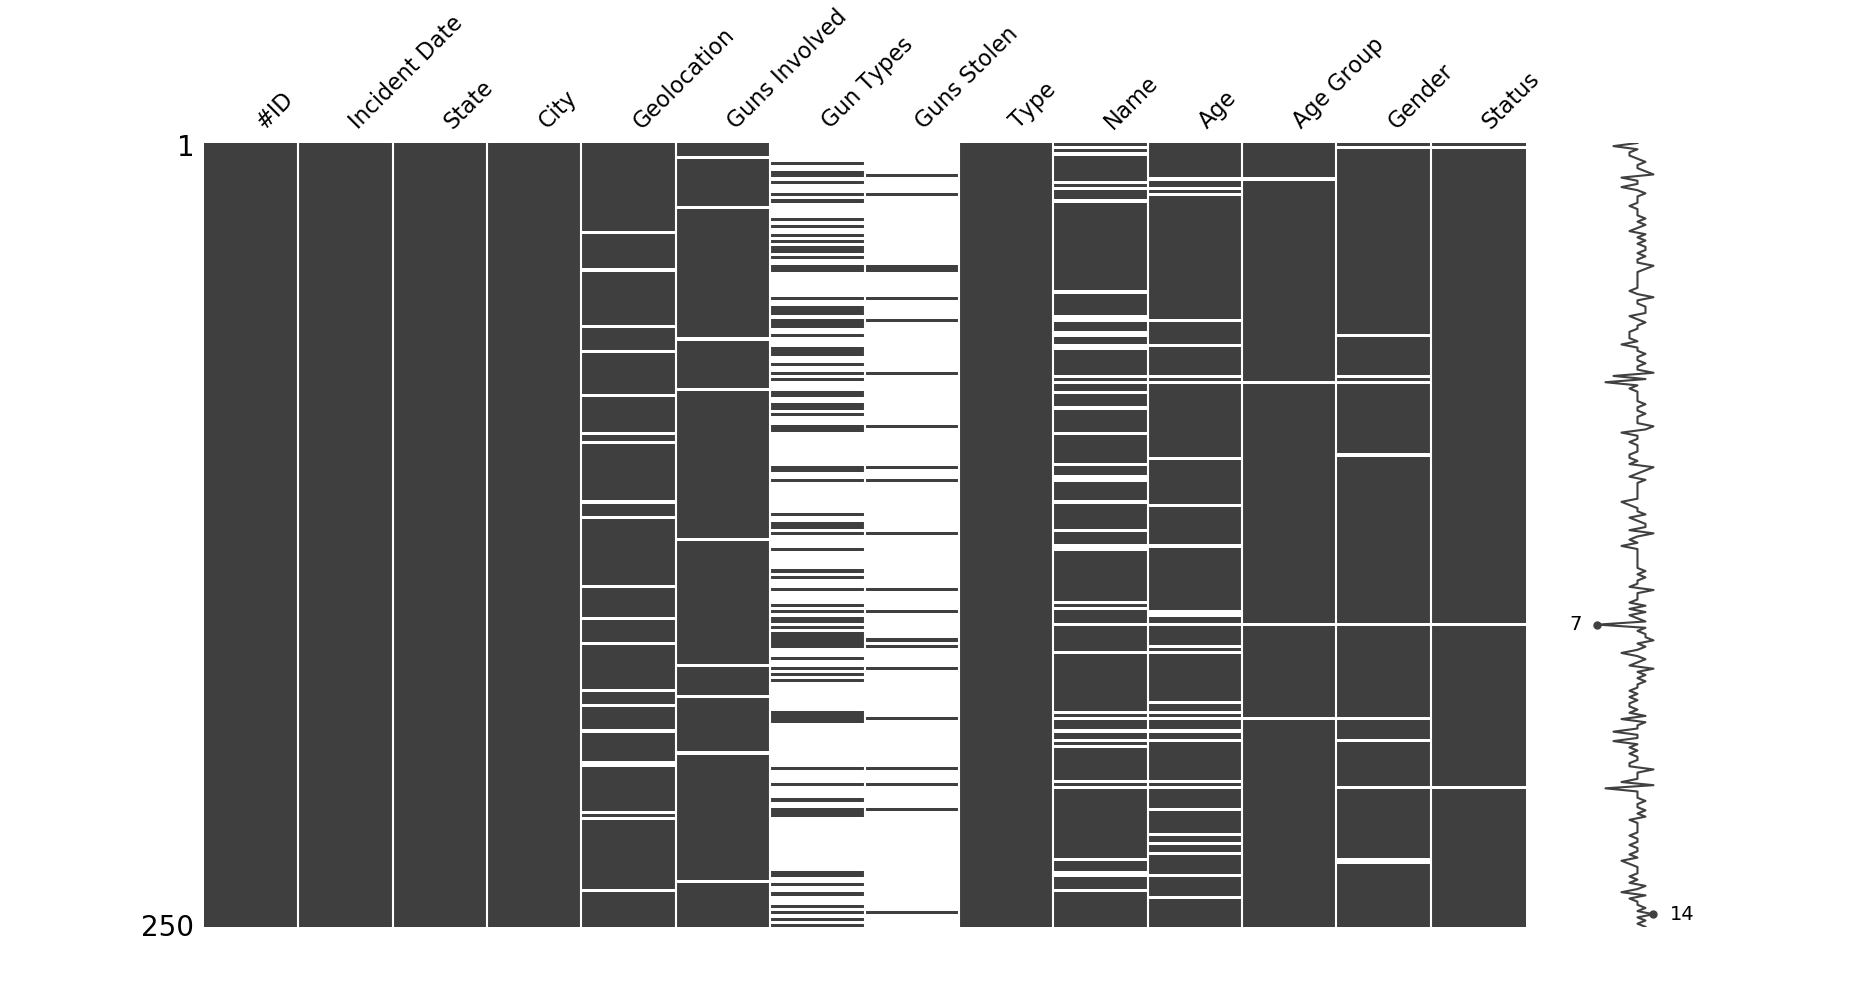
\includegraphics[width=\textwidth]
{missing_children_killed.png}
\caption{Children Killed Missing Values}
\end{figure}

\begin{figure}[H]
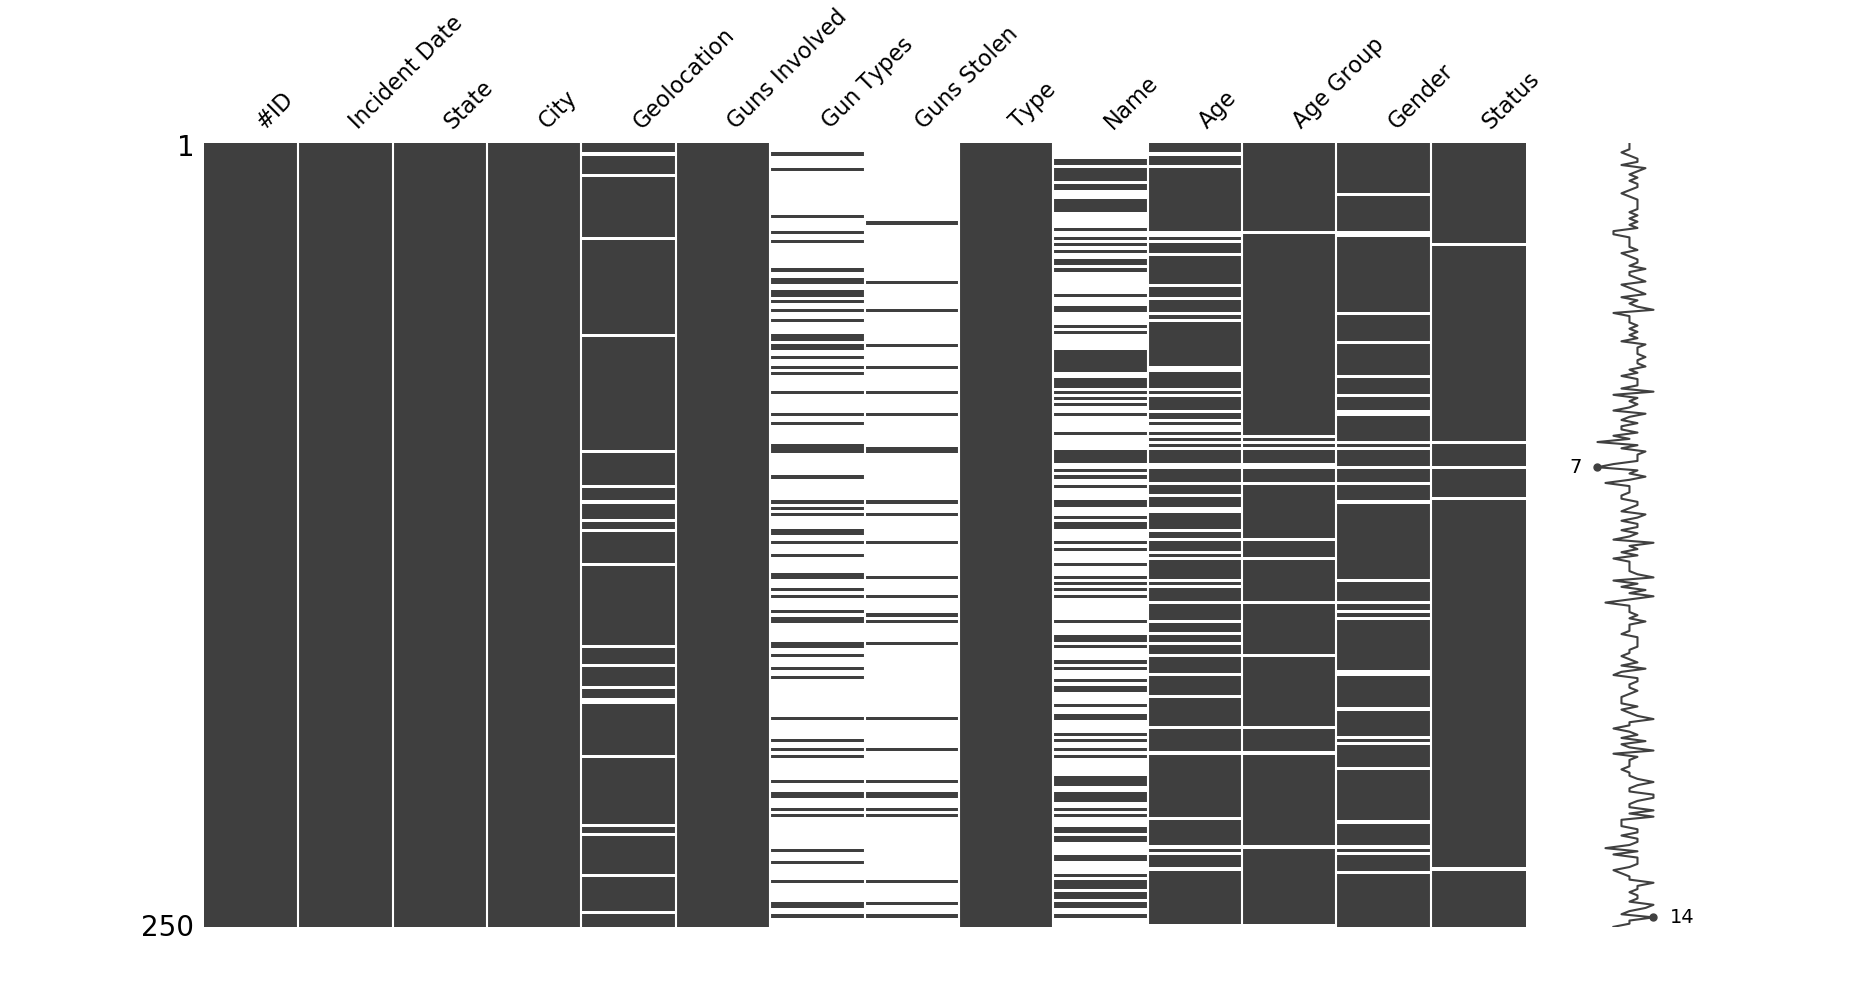
\includegraphics[width=\textwidth]{missing_children_injured.png}
\caption{Children Injured Missing Values}
\end{figure}

\begin{figure}[H]
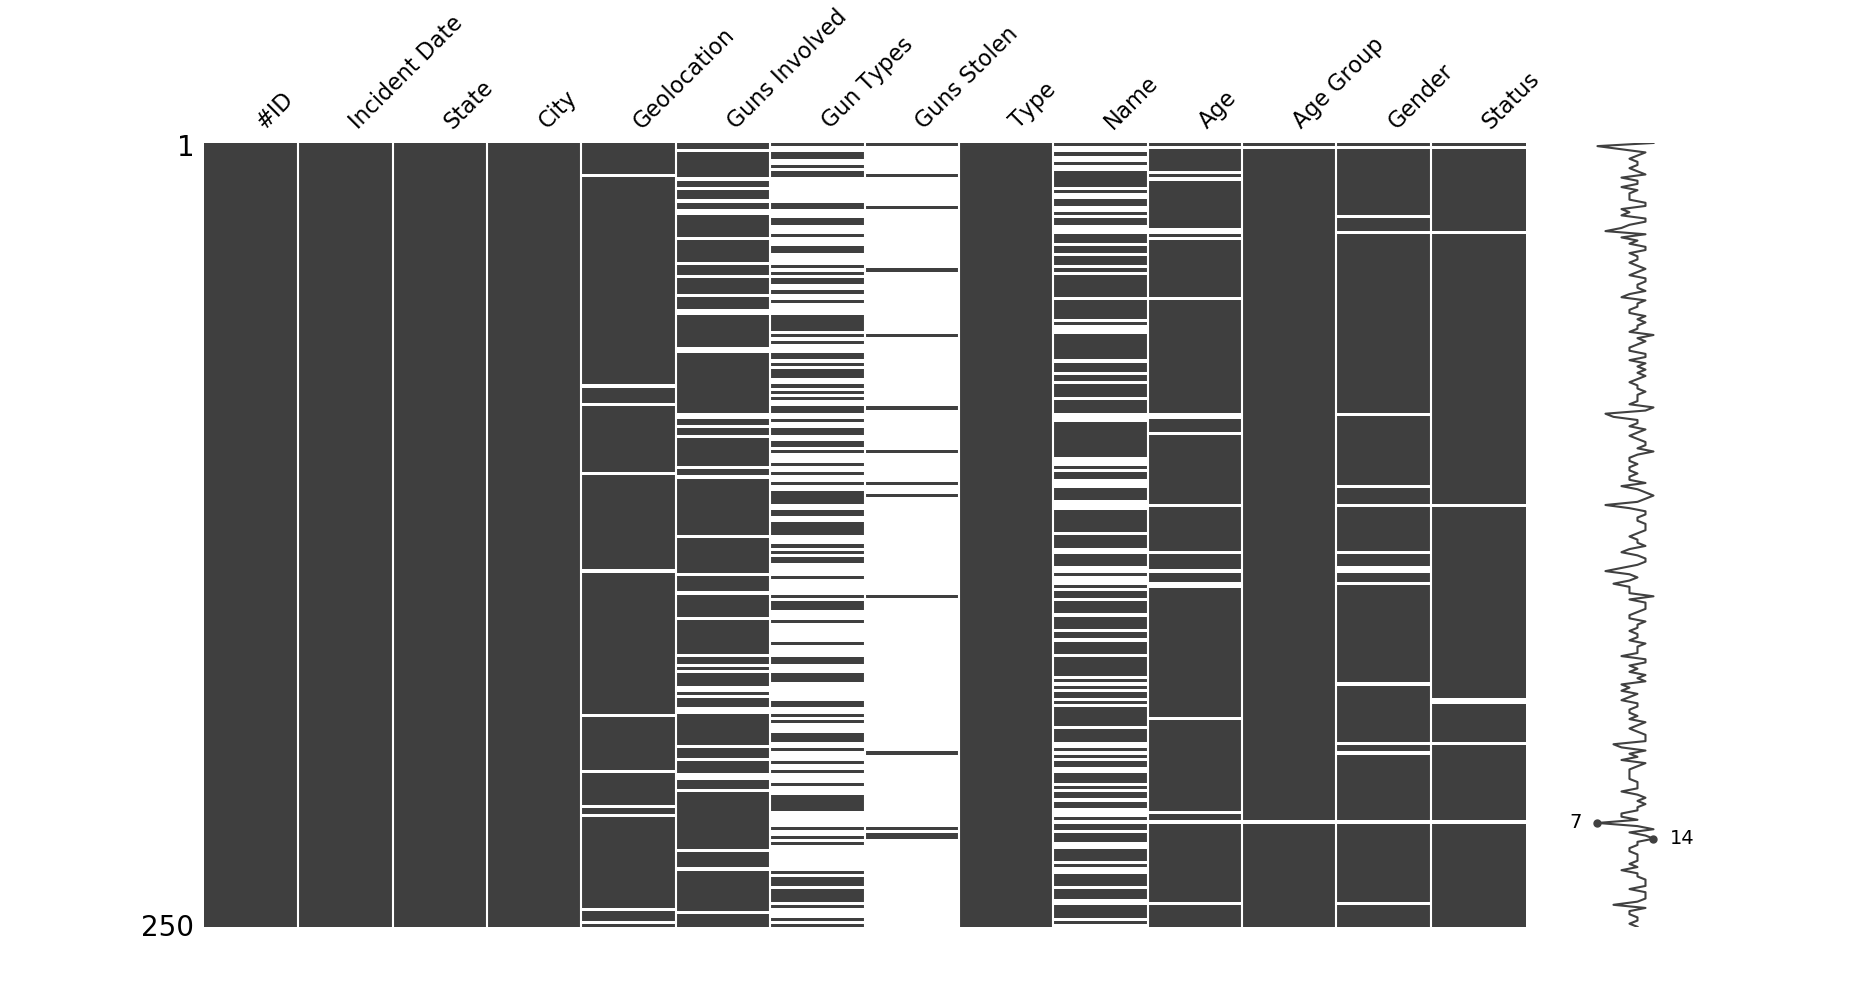
\includegraphics[width=\textwidth]{missing_accidental_deaths.png}
\caption{Accidental Deaths Missing Values}
\end{figure}

\begin{figure}[H]
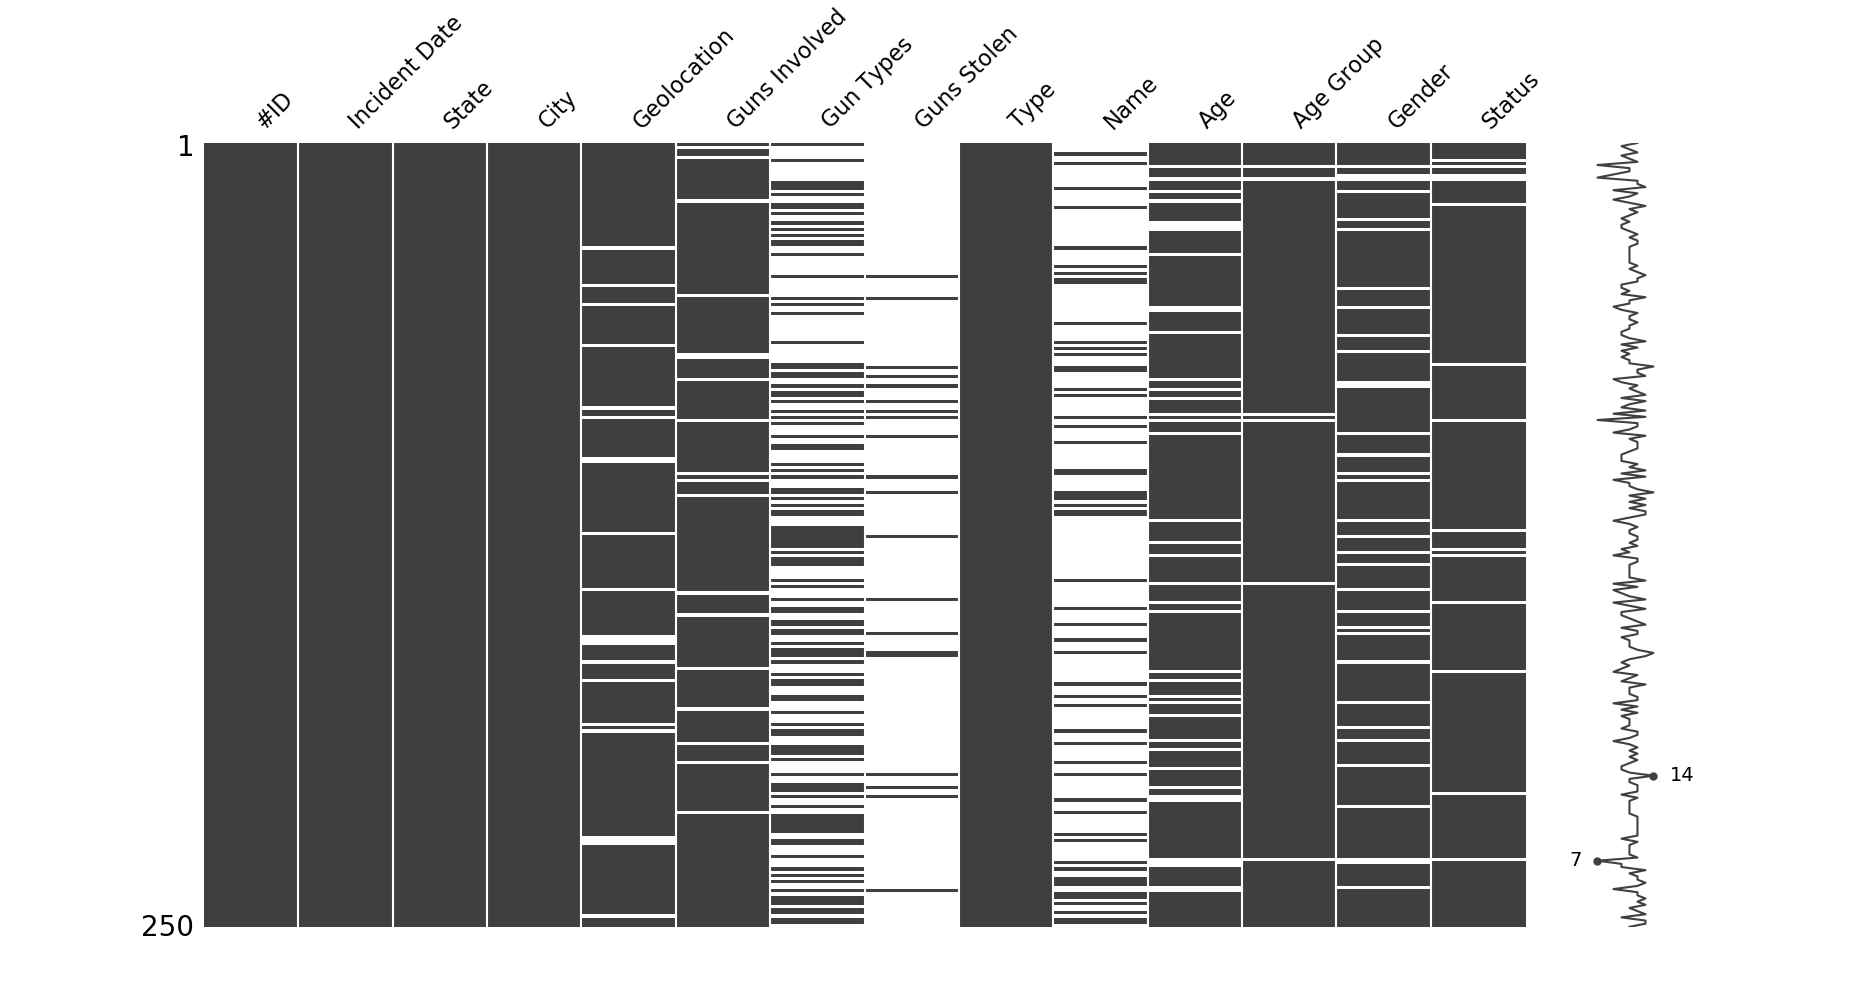
\includegraphics[width=\textwidth]{missing_accidental_injuries.png}
\caption{Accidental Injuries Missing Values}
\end{figure}

Praznine ozna\v cavaju nedostaju\' ce vrednosti. Kao \v sto smo i o\v cekivali, neki atributi nemaju nedostaju\' cih vrednosti kao \v sto je nazna\v ceno u tabeli \ref{table:atributi}, ali sada, za ostale vidimo koji imaju manje, a koji vi\v se.


\subsubsection{Geografska lokacija incidenta}
U podacima su nam obezbe\dj ene i geografska du\v zina i \v sirina, pa bi iz njihovog vizualnog prikaza moglo da se vidi u\v cestalost i raspore\dj enost na mapi. Te mogu\' cnosti pru\v za modul \textbf{geoplotlib} sa funkcijom \textit{kde} za prikaz mape gustine, ograni\v ceno na teritoriju USA gde su se dogodili incidenti:

\begin{lstlisting}
import geoplotlib
from geoplotlib.utils import read_csv, BoundingBox
import sys

args = sys.argv
if len(args) != 2:
    sys.exit(f"usage: ./{args[0]} /path/to/.csv")

data = read_csv(args[1])
geoplotlib.kde(data, 5, cut_below=1e-4, show_colorbar=False)
geoplotlib.set_bbox(BoundingBox.USA)
geoplotlib.show()
\end{lstlisting}

\begin{figure}[H]
\centering
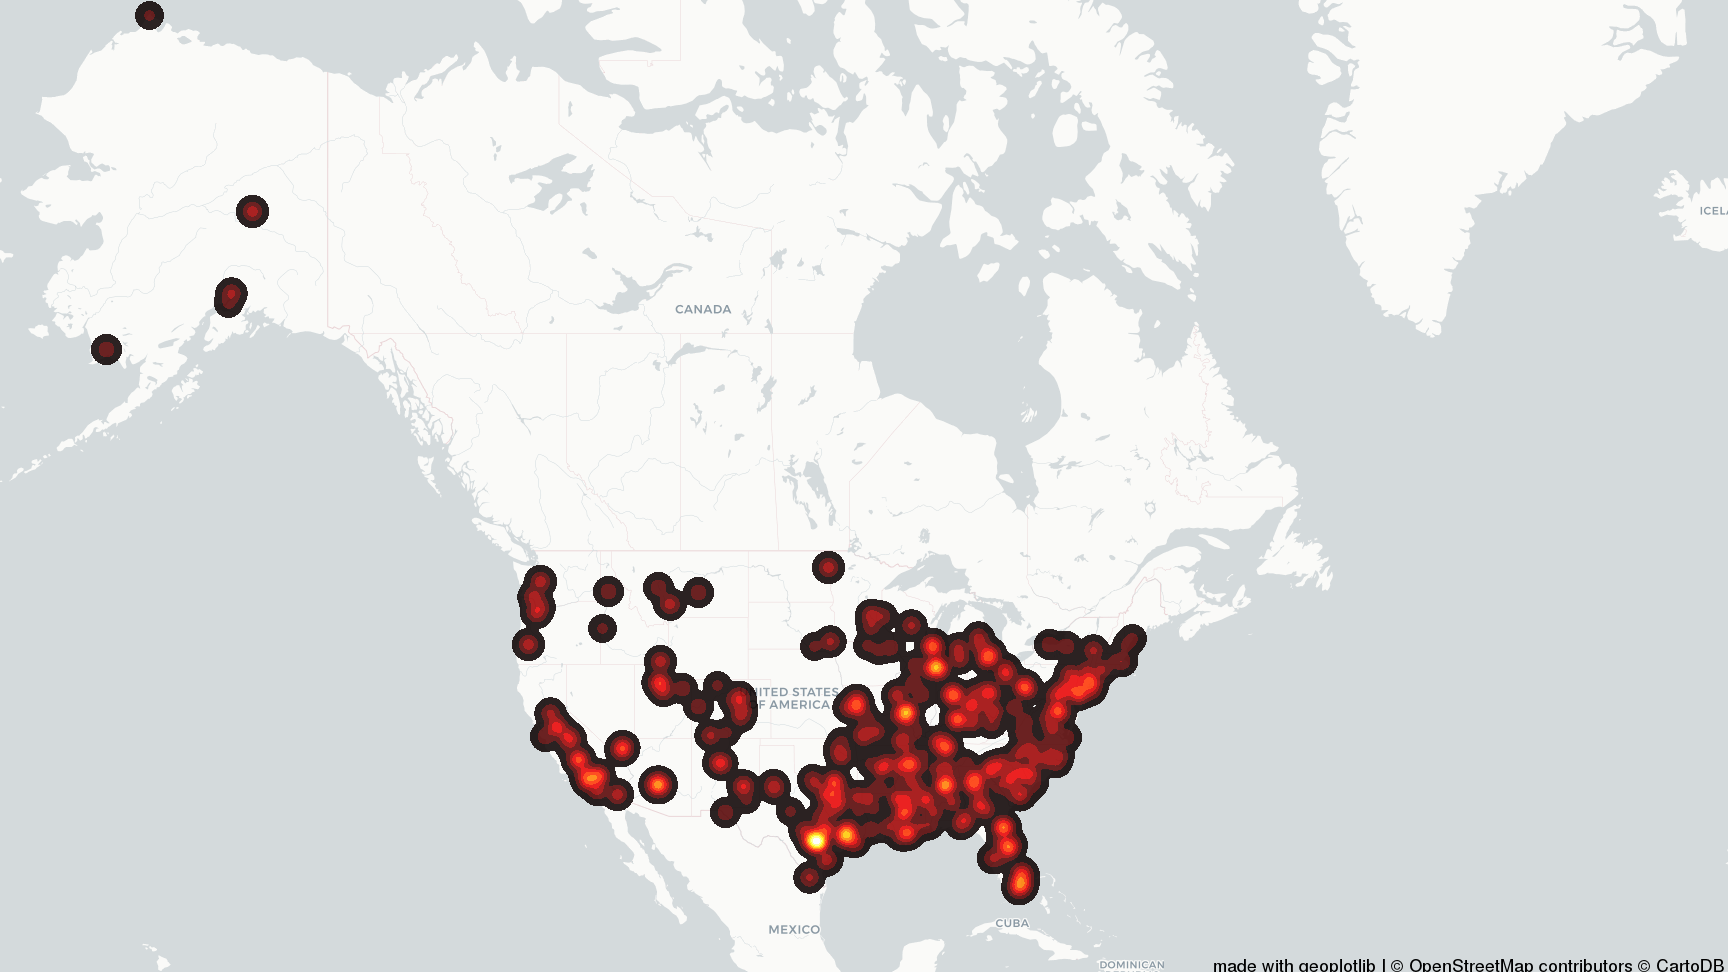
\includegraphics[width=0.8\textwidth]{geo_children_killed.png}
\label{fig:KilledGeo1}
\caption{Children Killed Geolocation}\hspace{0.5cm} \break
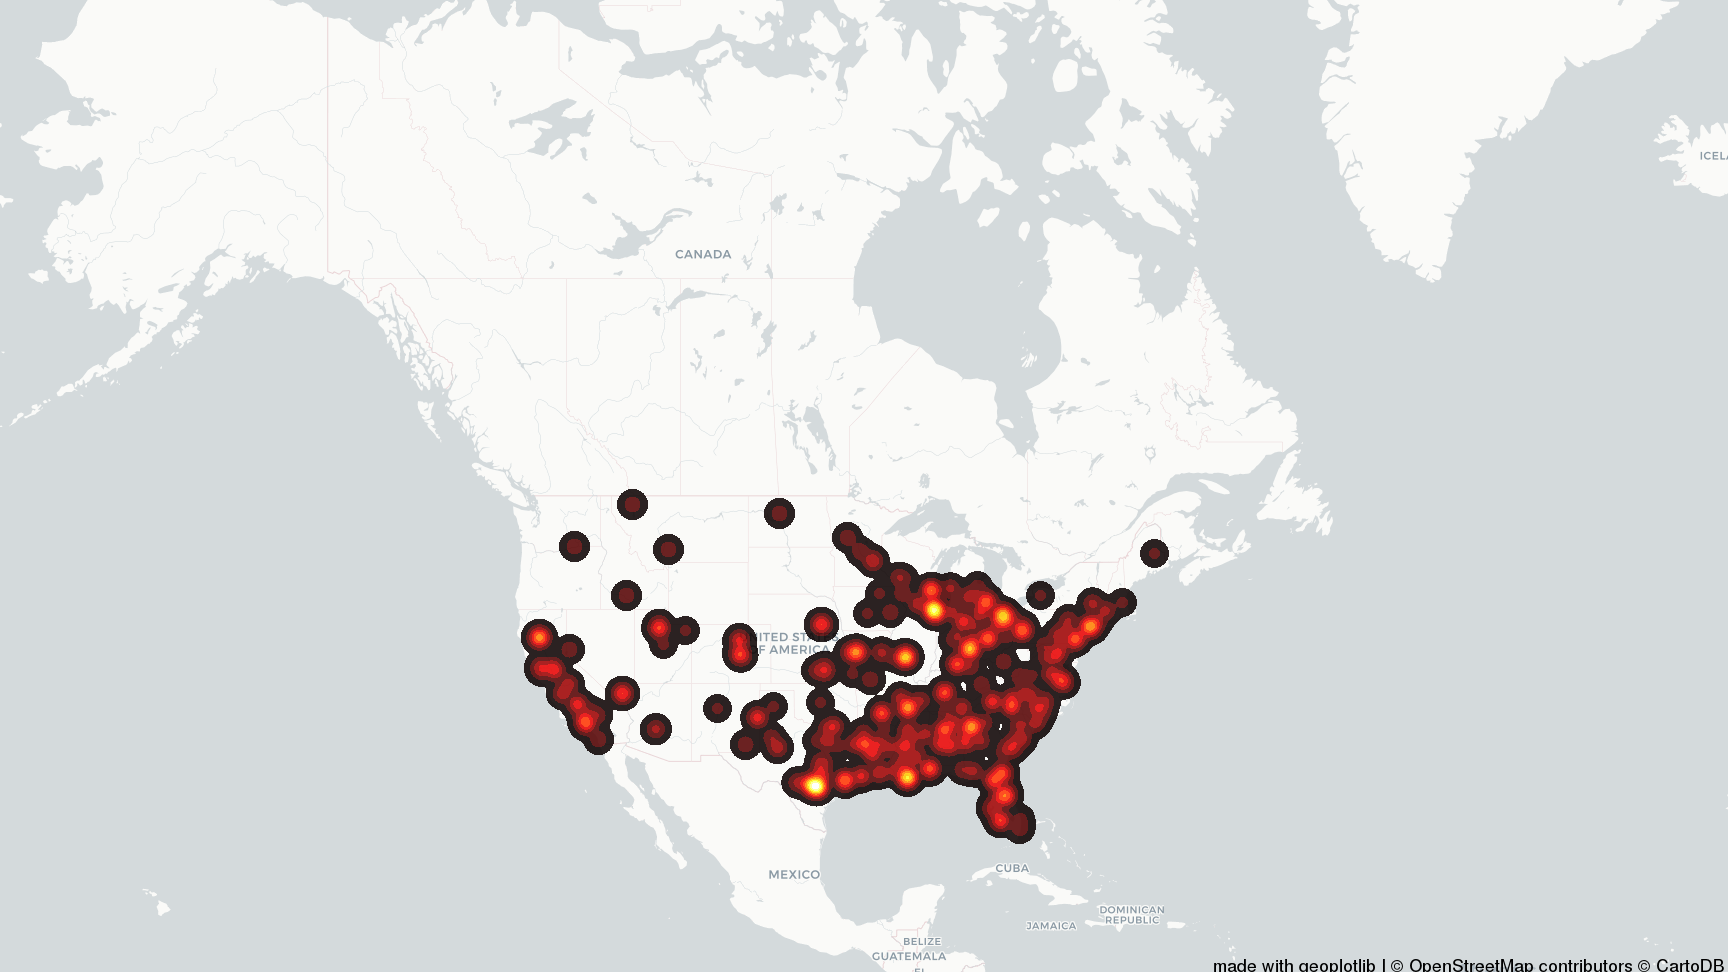
\includegraphics[width=0.8\textwidth]{geo_children_injured.png}
\label{fig:KilledGeo2}
\caption{Children Injured Geolocation}
\end{figure}

\begin{figure}[H]
\centering
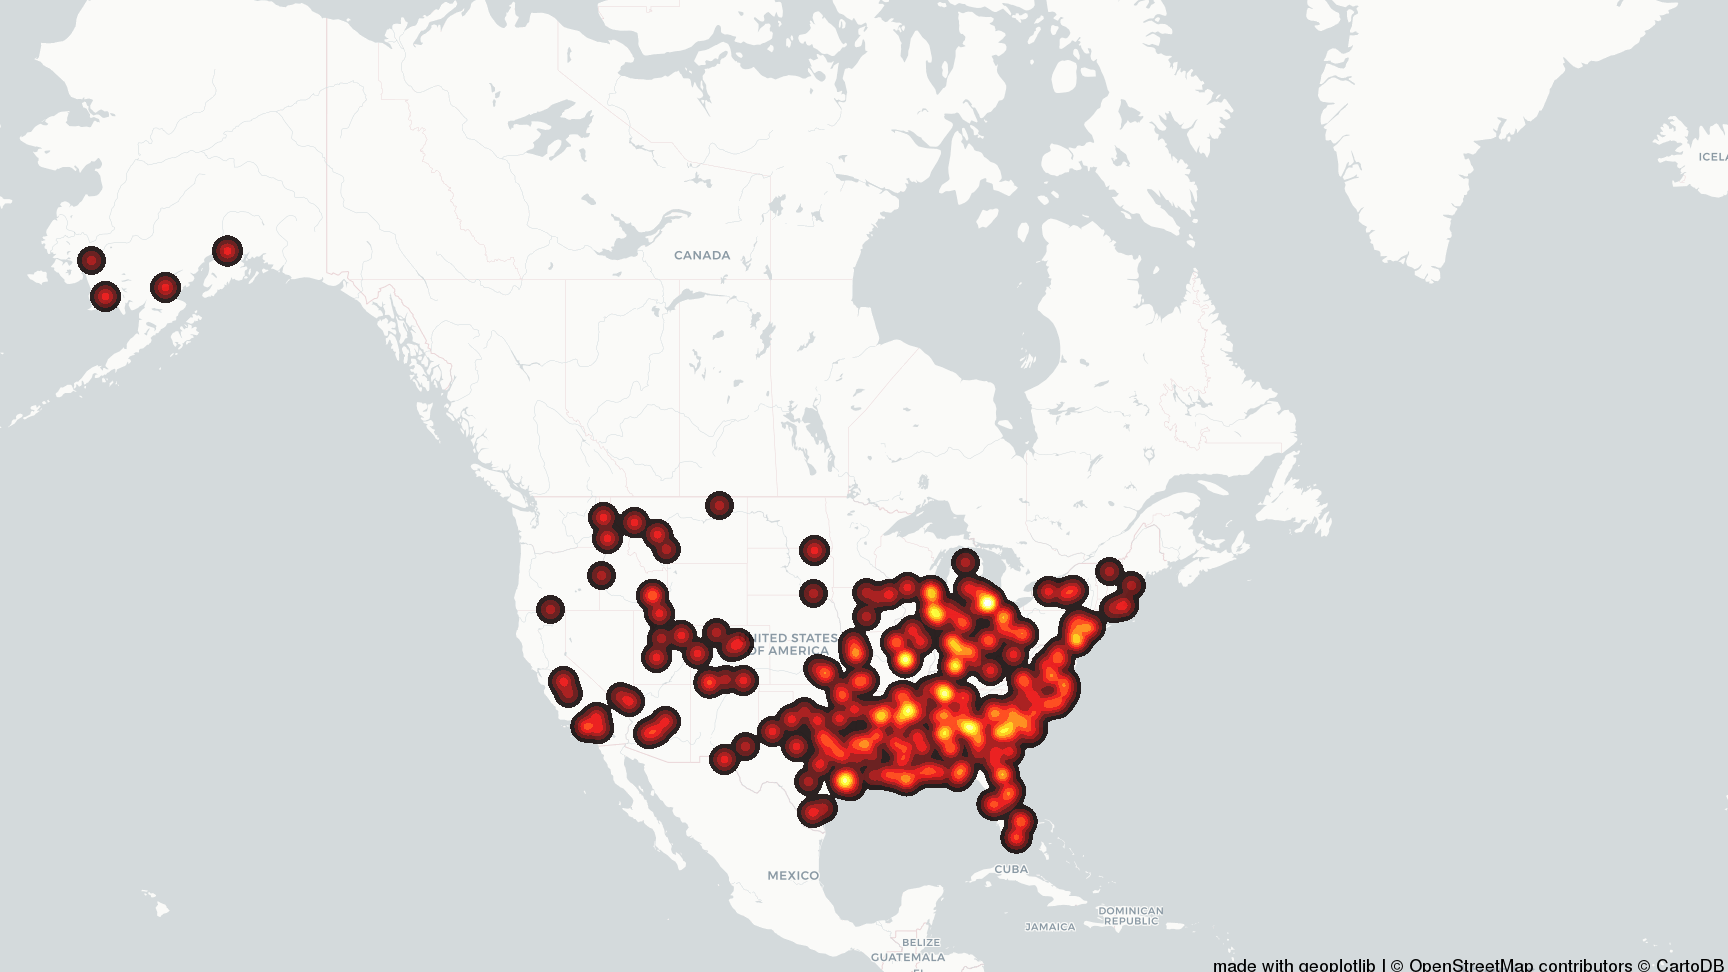
\includegraphics[width=0.8\textwidth]{geo_accidental_deaths.png}
\label{fig:AccidentalGeo1}
\caption{Accidental Deaths Geolocation}\hspace{0.5cm} 
\break
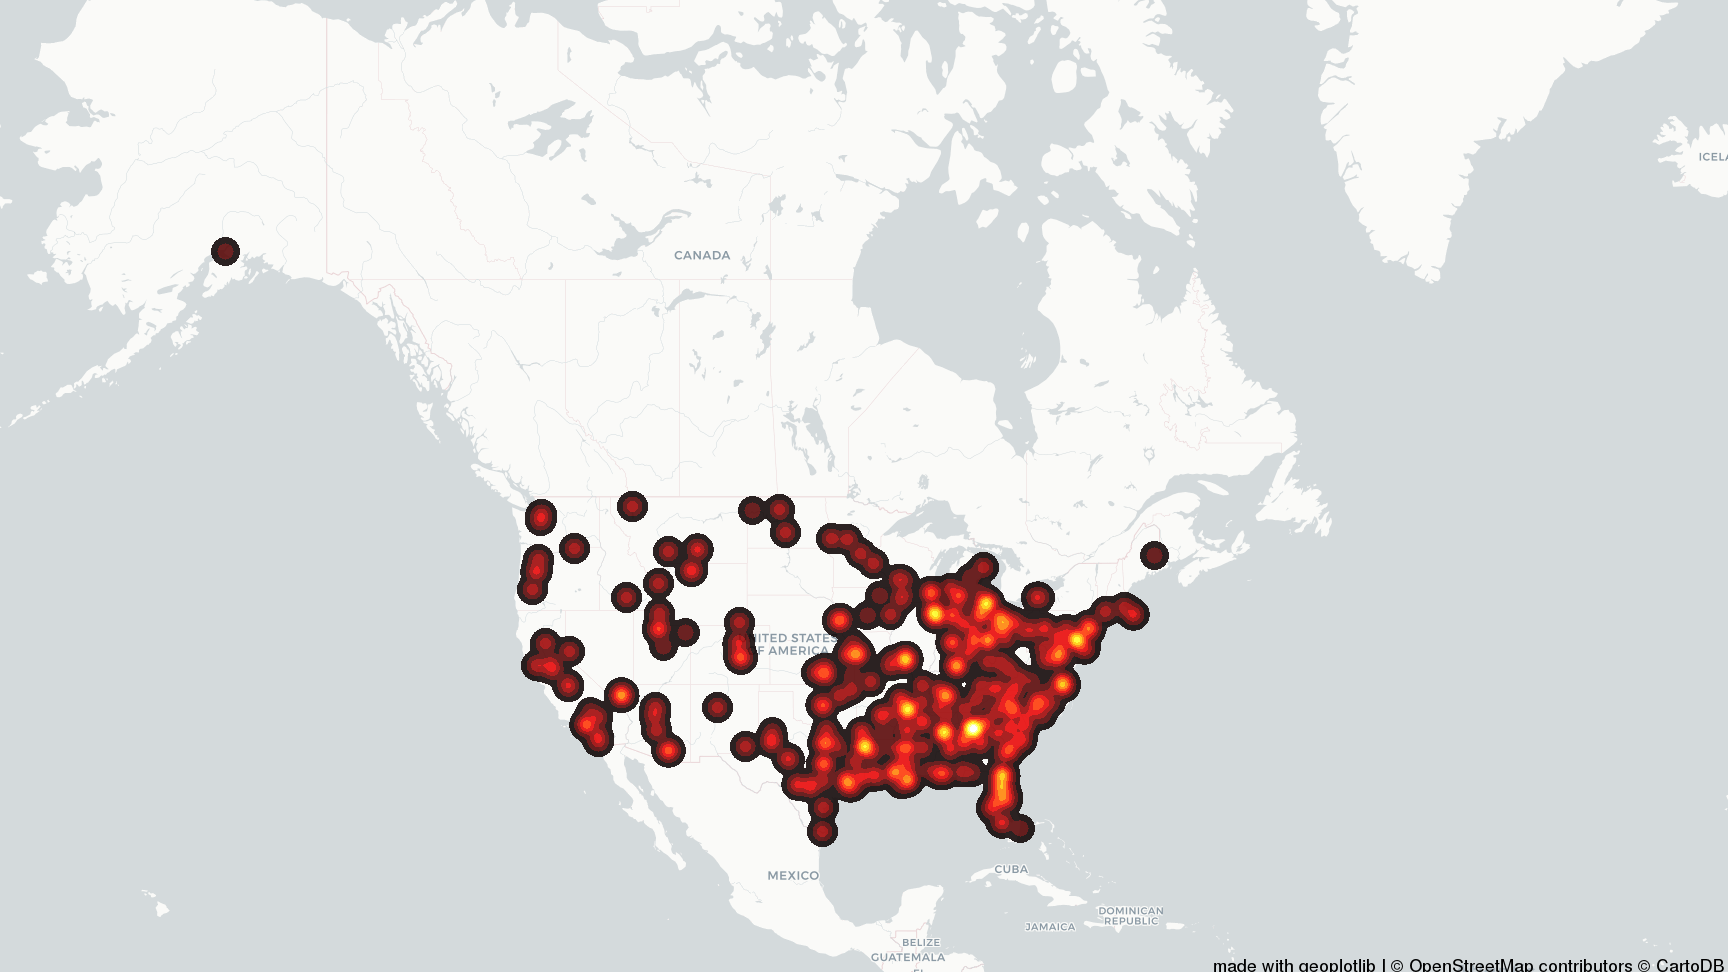
\includegraphics[width=0.8\textwidth]{geo_accidental_injuries.png}
\label{fig:AccidentalGeo2}
\caption{Accidental Injuries Geolocation}
\end{figure}

Tako\dj e, KNIME alatom mo\v zemo dobiti u kojoj dr\v zavi i u kom gradu imamo najvi\v se ubistava, \v sto potvr\dj uje prethodni prikaz na mapi. \footnote{Za nezgode pogledati originalni KNWF: children\_analysis}

\begin{figure}[H]
\centering
  \begin{minipage}[b]{0.3\textwidth}
    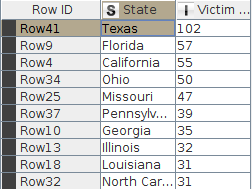
\includegraphics[width=\textwidth]{geoConfirm_state_childrenKI.png}
    \caption{Broj ubijenih po dr\v zavama}
  \end{minipage}
  \hfill
  \begin{minipage}[b]{0.3\textwidth}
    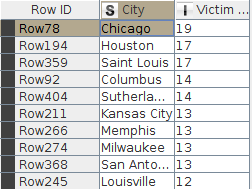
\includegraphics[width=\textwidth]{geoConfirm_city_childrenKI.png}
    \caption{Broj ubijenih po gradovima}
  \end{minipage}
\end{figure}



\subsection {Priprema podataka}

\subsubsection{Uvod}
U fazi pripreme podataka smo kreirali 4 odvojene datoteke koje koristimo u fazi obra\dj ivanja.\\
Prvi korak: grupisanje podataka po accidental deaths and injuries i killed and injured, zbog 
potencijalne analize izme\dj u te dve grupe i unutra\v snjih podgrupa.\\

Podatke u ove dve grupe smo grupisali po ID, s obzirom na to da nam je svaki doga\dj aj, odnosno svaka vrsta u tabeli imala svoj ID.\\

Kao \v sto vidimo iz tabele \ref{table:atributi} podaci nisu obra\dj eni, s obzirom na to da imamo nedostaju\' cih vrednosti u vi\v se atributa.\\

\subsubsection{\v Ci\v s\' cenje podataka}

Format u kojem smo dobili podatke (children\_killed.csv i children\_injured.csv) nije prilago\dj en za rad. Naime, imamo problem sa nedostaju\' cim vrednostima i normalizacijom.\break
 
S obzirom na to da radimo sa podacima koji nisu trivijalni, kao 
\v sto je na primer skup ta\v caka, gde mo\v zemo proceniti nedostaju\' ce vrednosti,
ovde smo se ipak odlu\v cili za varijantu eliminisanja problemati\v cnih instanci.\break

Imamo nedostaju\' ce vrednosti u slede\' cim atributima:
Guns Involved, Age. S obzirom da takvih instanci nema puno, eliminisali smo ih.

Tako\dj e imamo instance koje za atribute Gun Types, Gun Stolen i Gender imaju vrednosti N/A.
Za atribut Gender \' cemo takve instance isto ukloniti, jer ih ima malo, me\dj utim
kod Gun Types i Gun Stolen atributa prime\' cujemo da su skoro sve instance sa vrednostima N/A.
Tako ne\v sto nam ne\' ce pomo\' ci, zato \' cemo ukloniti te atribute kompletno.\break

Na\v s zadatak se sastoji u analizi smrti i povreda, konkretno dece, odnosno Age group - Children 0-11, ali mi u na\v sim podacima imamo i vi\v se od toga. Zato smo \v cvorom Rule-based Row Filter zadali pravilo prikazano na slici \ref{fig:filter}

\begin{figure}[H]
\centering
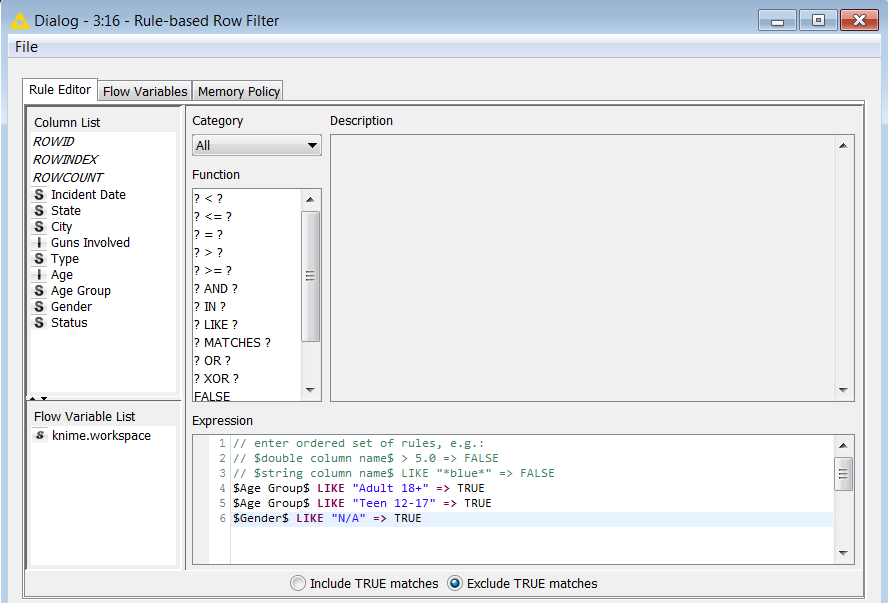
\includegraphics[width=0.76\textwidth]{dataPrepare_ruleBasedRowFilter.png}
\label{fig:filter}
\caption{Filtriranje podataka}
\end{figure}

Time smo se oslobodili nepotrebnih instanci.
Sada kada smo to uradili, mo\v zemo ukloniti i atribut Age group.\break

Kada izvr\v simo istu pripremu nad podacima accidental\_deaths.csv i accidental\_injuries.csv vidimo da nam atribut Guns Involved za sve
instance ima vrednost 1, \v sto nije slu\v caj od pre.


\subsubsection{Prikaz}
Nakon sre\dj ivanja podataka u \textit{Knime-u} mo\v zemo prikazati dobijene rezultate u formi \textit{Scatter Matrix} i \textit{Pie chart}, kao i statisti\v cki prikaz podataka sa \textit{Box Plot} i \textit{Statistics}.

\begin{figure}[H]
\centering
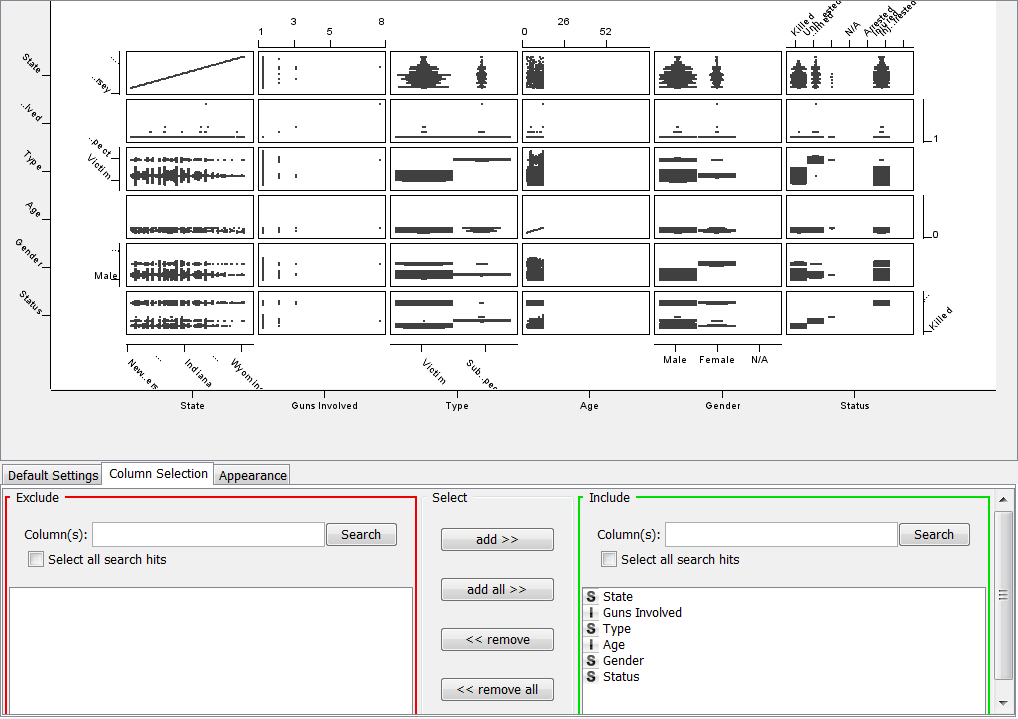
\includegraphics[width=0.7\textwidth]{visualisation_scatterMatrix_accidentalDI.png}
\caption{Accidental Deaths and Injuries Scatter Matrix}\hspace{0.5cm} \break
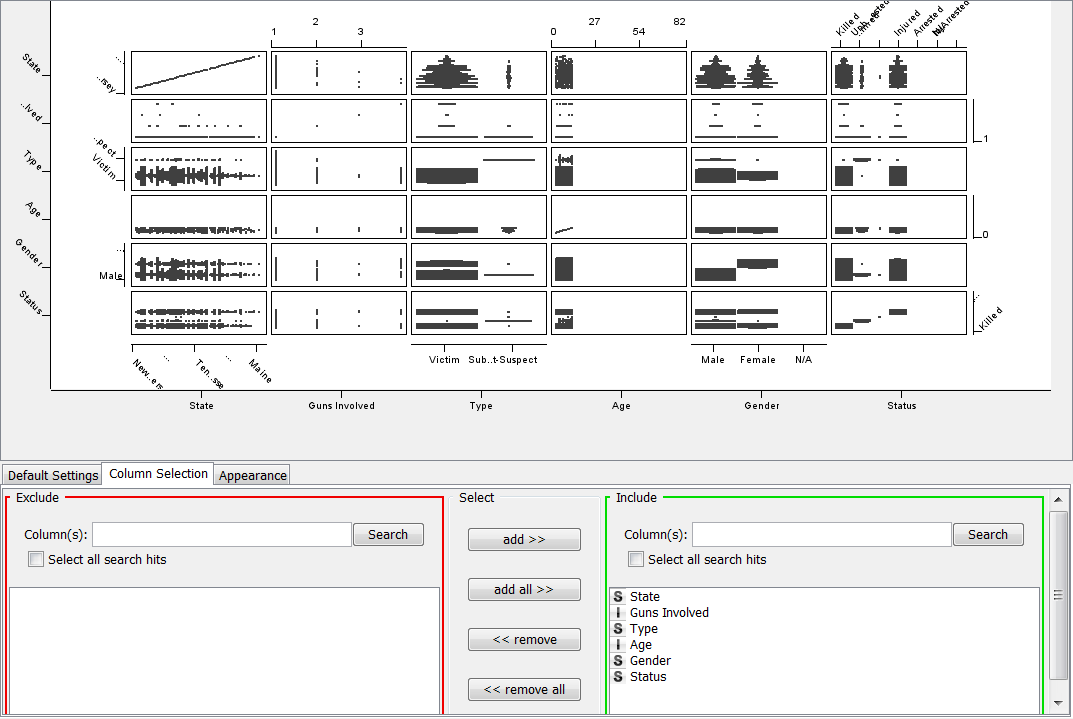
\includegraphics[width=0.7\textwidth]{visualisation_scatterMatrix_childrenKI.png}
\caption{Children Killed and Injured Scatter Matrix}
\end{figure}

\newpage
Sa prilo\v zenih grafikona uo\v cavamo sli\v cnost procenata povre\dj ene dece za obe grupacije, \v sto je oko 43\%, dok mo\v zemo primetiti znatnu razliku u procentima ubijene dece za ove grupacije. Razlikuju se do na 15\%. Interesantno je primetiti da je mnogo vi\v se slu\v cajnih smrti nego ubistava.
Me\dj utim mo\v zemo zaklju\v citi da je odnos uhap\v senih i neuhap\v senih po\v cinitelja znatno razli\v cit i to 0.21\%, 0.81\%, respektivno. \v Sto zna\v ci da su po\v cinitelji zlo\v cina i privedini.
\begin{figure}[H]
\centering
  \begin{minipage}[b]{0.45\textwidth}
    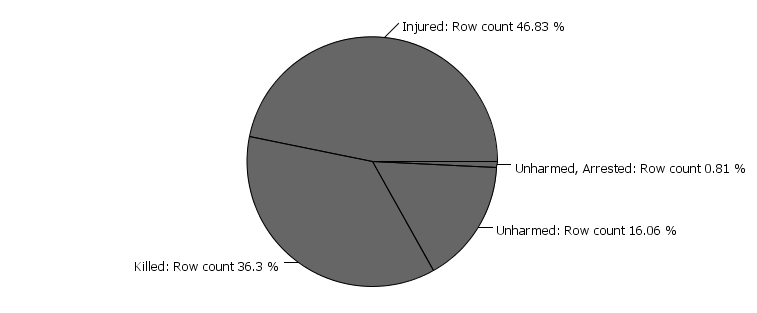
\includegraphics[width=\textwidth]{visualisation_PieChart_accidentalDI.png}
    \caption{Accidental Deaths and Injuries Pie Chart}
  \end{minipage}
  \hfill
  \begin{minipage}[b]{0.45\textwidth}
    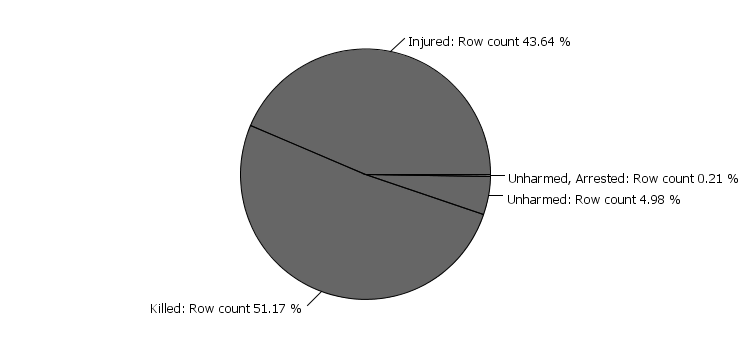
\includegraphics[width=\textwidth]{visualisation_PieChart_childrenKI.png}
    \caption{Children Killed and Injured Pie Chart}
  \end{minipage}
\end{figure}

Pogledajmo sada slede\' ce prikaze \textit{Box Plot}. Na slici \ref{fig:ADboxplot} imamo elemente van granica u atributu \textit{State}. Ali ovo je i o\v cekivano jer smo u geografskom prikazu lokacije incidenata po\v cetnih podataka \footnote{Pogledati geografski prikaz na slikama: \ref{fig:KilledGeo1}, \ref{fig:KilledGeo2}, \ref{fig:AccidentalGeo1} i \ref{fig:AccidentalGeo2}}
videli izme\v stenost nekoliko instanci na podru\v ciju Aljaske, dok u skupu \textit{Accidental Deaths and Injuries} nemamo elemenata van granica. 

\begin{figure}[H]
\centering
  \begin{minipage}[b]{0.45\textwidth}
    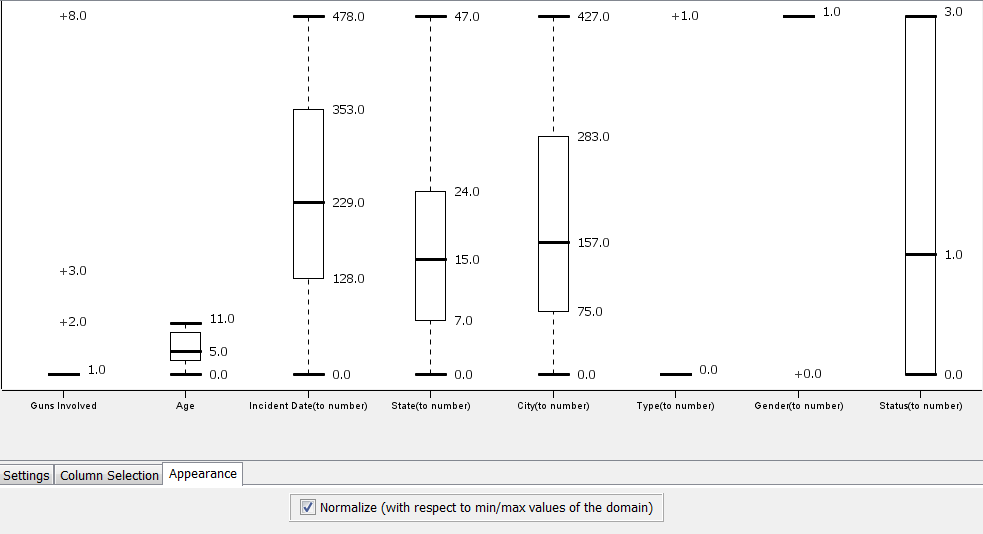
\includegraphics[width=\textwidth]{visualisation_boxplot_accidentalDI.png}
    \caption{Accidental Deaths and Injuries Box Plot}
    \label{fig:ADboxplot}
  \end{minipage}
  \hfill
  \begin{minipage}[b]{0.45\textwidth}
    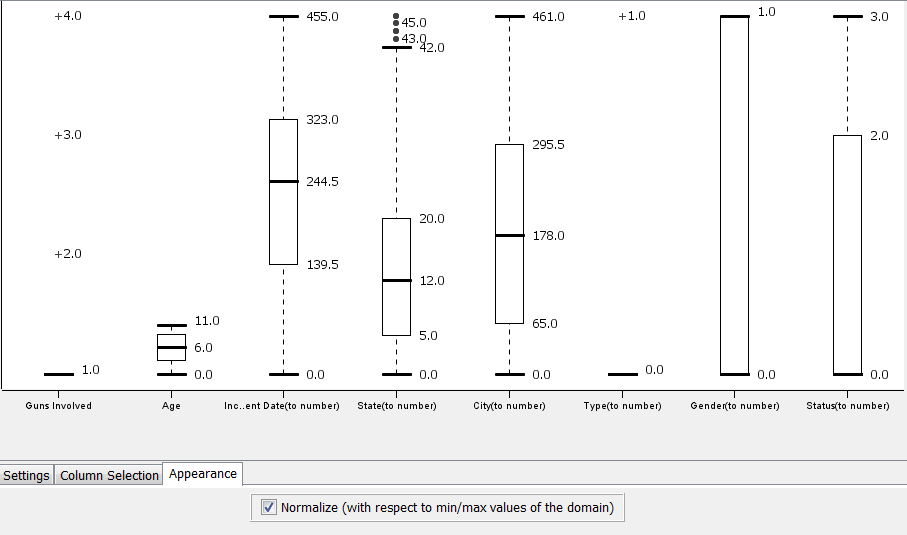
\includegraphics[width=\textwidth]{visualisation_boxplot_childrenKI.png}
    \caption{Children Killed and Injured Box Plot}
    \label{fig:KIboxplot}
  \end{minipage}
\end{figure}

\newpage
Tako\dj e mo\v zemo posmatrati linearnu korelaciju izmedju atributa, i ono \v sto mo\v zemo primetiti da je za obe grupe koje analiziramo uo\v cena korelacija izmedju atributa State i Type, \v sto zna\v ci da bismo mogli eliminisati jedan atribut, ali jednostavnije je da to u ovom trenutku ne radimo.
\begin{figure}[H]
\centering
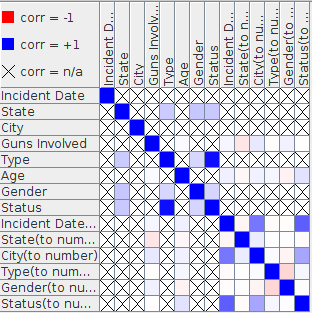
\includegraphics[width=0.4\textwidth]{visualisation_linearCorrelation_childrenKI.png}
\caption{Korelacija za Children Killed and Injured}
\end{figure}

\section {Analiti\v cka obrada i algoritmi}
\subsection {Pravila pridru\v zivanja}

Prvi primenjen algoritam je Apriori algoritam, koji spada u algoritam za pravila pridru\v zivanja. Cilj nam je da vidimo imamo li nekih interesantnih pravila. Mera interesantnosti za na\v se podatke mo\v ze biti Lift mera.\break


\textbf{Prvi na\v cin}: kori\v s\' cenje KNIME cvora \textit{Apriori(3.7)}, 
sa slede\' cim pode\v savanjima:\\
minimalna podrska = 0.2\\
metricType = Confidence od mogu\' cih Lift, Conviction.\hspace{0.5cm} \break

Zapravo, menjanjem ovih vrednosti (pove\' cavanjem/smanjenjem 
minimalne podr\v ske...) nemamo interesantnije podatke.
Dobijen je slede\' ci izlaz:
\begin{figure}[H]
\centering
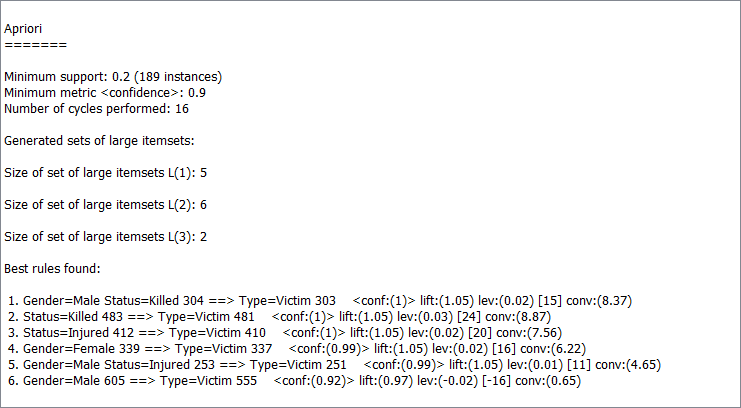
\includegraphics[width=0.67\textwidth]{aprioriAlgorithm_childrenKI.png}
\caption{Children Killed and Injured Apriori}
\end{figure}

Kako konkretno izgleda \v cvor ne mo\v zemo prikazati jer ne postoji taj \v cvor na novijoj verziji KNIME alata, ve\' c samo na virtualnoj ma\v sini pri staroj verziji.\break

\textbf{Drugi na\v cin}: Ru\v cno kreiranje \v cestih skupova stavki i pravila pridru\v zivanja uz pomo\' c 
\v cvora \textit{Association Rule Learner}, iz kojeg mo\v zemo zaklju\v citi slede\' ce: \break

Broj \v cestih skupova = 23\\
Najmanja podr\v ska = 0.314\\
Najve\' ca podr\v ska = 0.962\\

\begin{figure}[H]
\centering
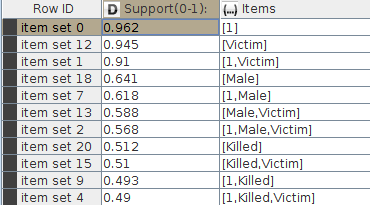
\includegraphics[width=0.4\textwidth]{aprioriAlgorithm_commonSubset_childrenKI.png}
\caption{\v Cesti skupovi stavki za Children Killed}
\end{figure}

Broj pravila pridru\v zivanja = 54\\
Najmanja podr\v ska = 0.253\\
Najve\' ca podr\v ska = 0.91\\

\begin{figure}[H]
\centering
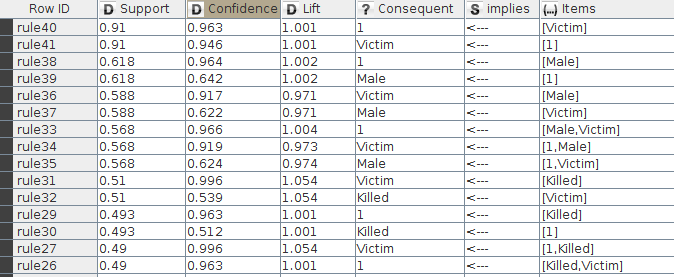
\includegraphics[width=0.7\textwidth]{associationRules_ChildrenKI.png}
\caption{Pravila pridru\v zivanja za Children Killed and Injured}
\end{figure}

Neka od pravila su:\\
	\textit{Type} Victim =$>$ \textit{Guns Involved} 1 sa podr\v skom \textit{0.91} i lift merom 1.001.\\  
	\textit{Gender} Male =$>$ \textit{Guns Involved} 1 sa podr\v skom \textit{0.618} i lift merom 1.002.\break
	
Vidimo da je Lift mera oko 1 i pravila su krajnje trivijalna, naime ako je neko \v zrtva logi\v cno je da je u ubistvu u\v cestvovalo bar jedno oru\v zje. Iz ovoga mo\v zemo 
zaklju\v citi da dobijena pravila nisu zanimljiva.\break
	
Sli\v cni rezultati su dobijeni primenom algoritma nad podacima \textit{accidental\_deaths} i \textit{accidental\_injuries}. Dobijeno je manje \v cestih skupova i pravila pridru\v zivanja, takodje je najve\' ca podr\v ska manja od malopre.

\subsection{Klasterovanje}
Klasterovanje spada u tehniku prepoznavanja klastera bez poznavanja izlaza.
Zato \' cemo videti, da se klasifikacija pona\v sa mnogo bolje od klasterovanja.

\v Zelimo da nam ciljni atribut bude atribut Status. Odnosno, \v zelimo da na osnovu svih podataka zaklju\v cimo da li je osoba ubijena, povre\dj ena, uhap\v sena itd.\break

Zaklju\v cak koji smo doneli na osnovu slede\' ca tri algoritma je da ni u jednom nismo uspeli da klasterujemo podatke i dobijemo o\v cekivani status. 


\subsubsection{K-sredina}	
Ova tehinka klasterovanja se zasniva na centru i particionisanju, koja poku\v sava da pronadje korisni\v cki definisan broj klastera. 
S obzirom da je najve\' ca mana ovog algoritma koji broj klastera uzeti, mi \' cemo napraviti petlju gde \' cemo taj parametar klastera, odnosno k, pro\v setati kroz mogu\' ce vrednosti od 2 do naprimer 7 i videti \v sta time dobijamo preko Scatter-Plot-a.\break

S obzirom da K-sredina radi samo sa numeri\v ckim podacima, potrebno je konvertovati kategori\v cke podatke i normalizovati.\break

\begin{figure}[H]
\centering
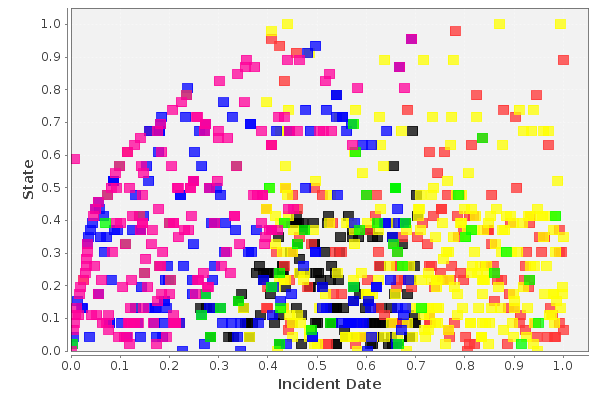
\includegraphics[width=0.7\textwidth]{kMeans_6.png}
\caption{K-sredina za broj klastera 6}
\end{figure}

Eksportovali smo rezultate klasterovanja u folder kMeans\_childrenKI iz kojeg mo\v zemo zaklju\v citi da se ni\v sta nije klasterovalo kao \v sto bismo o\v cekivali, svi klasteri su izme\v sani za svako k (koje predstavlja broj klastera). 

\newpage
\subsubsection{Hijerarhijsko klasterovanje}
Hijerarhijskim klasterovanjem, kao i kod K najbli\v zih suseda, nismo dobili dobro klasterovane podatke, kao \v sto mo\v zemo videti u prilogu.
\begin{figure}[H]
\centering
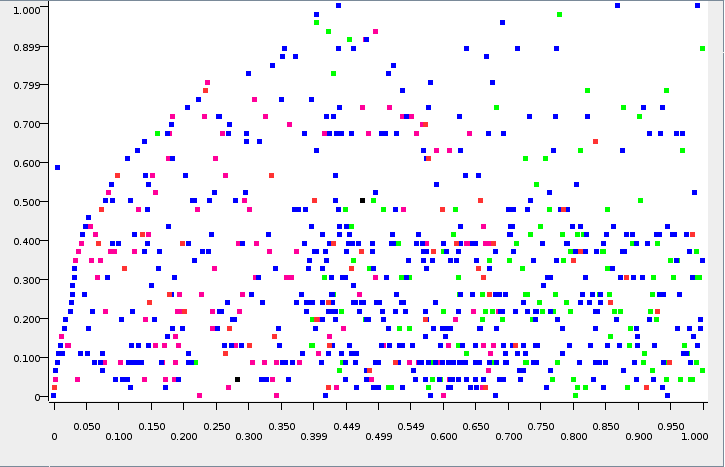
\includegraphics[width=0.7\textwidth]{hierarchicalClustering_childrenKI.png}
\caption{Hijerarhijsko klasterovanje za broj klastera 5}
\end{figure}


\subsubsection{DBSCAN}
Jo\v s jedan algoritam klasterovanja je DBSCAN klasterovanje. 
Stavili smo petlje, u nadi da \' ce se pokazati bolje od ostalih algoritama klasterovanja,
ali iz foldera dbscan\_childrenKI u kojem su ekspportovane slike za razli\v cite brojeve epsilon i minpts, vidimo da je sve klasterovano u jedan klaster.\\ 
Kori\v s\' ceni parametri: 
$epsilon \in [1..0.5..3]$ i $minpts \in [3,5]$
\begin{figure}[H]
\centering
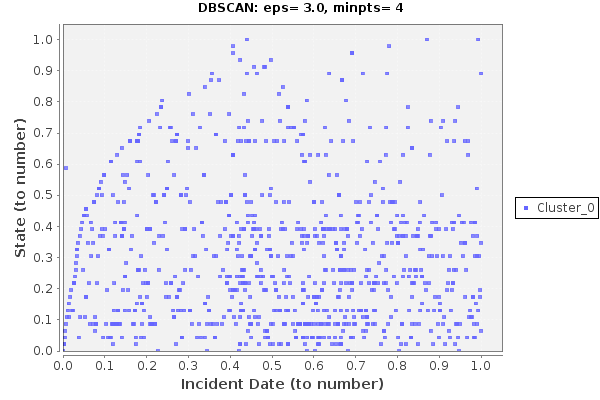
\includegraphics[width=0.7\textwidth]{dbscan_eps_3_0_minpts_4.png}
\caption{DBSCAN}
\end{figure}


\subsection{Klasifikacija}
U svim algoritmima nam je i dalje cilj da se poga\dj a status, ali s obzirom da se radi o klasifikaciji, uzima se u obzir i \v zeljeni izlaz.\\
U svim algoritmima se prvo podaci moraju razdvojiti na trening (70\%) i test skup, kori\v s\' cenjem slojevitog uzorkovanja \textit{(engl. stratified sampling)} pomo\' cu KNIME \v cvora \textit{Partitioning}.\break

Zaklju\v cak iz svih navedenih algoritama da su se najbolje pokazali algoritmi K najbli\v zih suseda i Neuronske mre\v ze sa precizno\v s\' cu na test skupu \v cak 85\%.

\subsubsection{Stabla odlu\v civanja}
Prvi algoritam klasifikacije koji smo primenili je stablo odlu\v civanja.
Kori\v s\' cena mera kvaliteta je Gini indeks.

Ono \v sto mo\v zemo zaklju\v citi je da je algoritam sveo stablo na dubinu 2 \v sto je dobro, jer na osnovu jednog atributa (Type) mo\v zemo zakljuciti status. Naime, ako je 
osoba \v zrtva onda je ona i ubijena (54\%), a ako je osumnji\v cen onda je i nepovre\dj en (\v cak 89\%).\break

\begin{figure}[H]
\centering
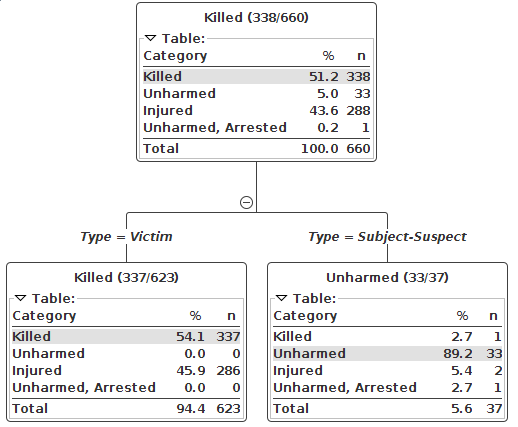
\includegraphics[width=0.7\textwidth]{treeClassifier_tree_childrenKI.png}
\caption{Stablo odlu\v civanja}
\end{figure}

Ali, na osnovu preciznosti mo\v zemo re\' ci da ovo ba\v i nije merodavno klasifikovano, jer je preciznost na test skupu kao i na trening skupu oko 50\%.

\begin{figure}[H]
\centering
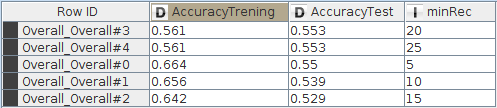
\includegraphics[width=0.7\textwidth]
{treeClassifier_accr_childrenKI.png}
\caption{Preciznosti za test i trening skup za stablo odlu\v civanja}
\end{figure}

Na slede\' coj slici imamo prikazanu matricu konfuzije za test skup. Iz nje mo\v zemo zaklju\v citi da je atribut killed klasifikovan veoma dobro, dok je za atribut injured potpuno pogre\v sno klasifikovao. Svi koji treba da budu povre\dj eni su klasifikovani kao ubijeni.

\begin{figure}[H]
\centering
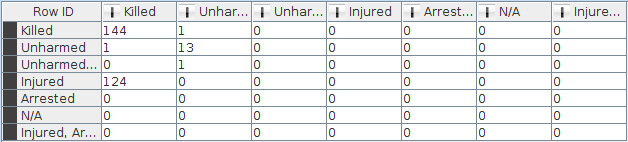
\includegraphics[width=0.7\textwidth]{treeClassifier_confussionMatrix_childrenKI.png}
\caption{Matrica konfuzije za test skup za stablo odlu\v civanja}
\end{figure}


Ako podesimo u algoritmu parametar da se stablo mora razviti po nekom atributu, na primer state, dobijamo slede\' ce stablo.
Vidimo da nije mogao kao malo pre algoritam u jednom koraku da zaklju\v ci ciljni status, ve\'c se negde grana po atributu godine, i da preciznost nije bolja.
\begin{figure}[H]
\centering
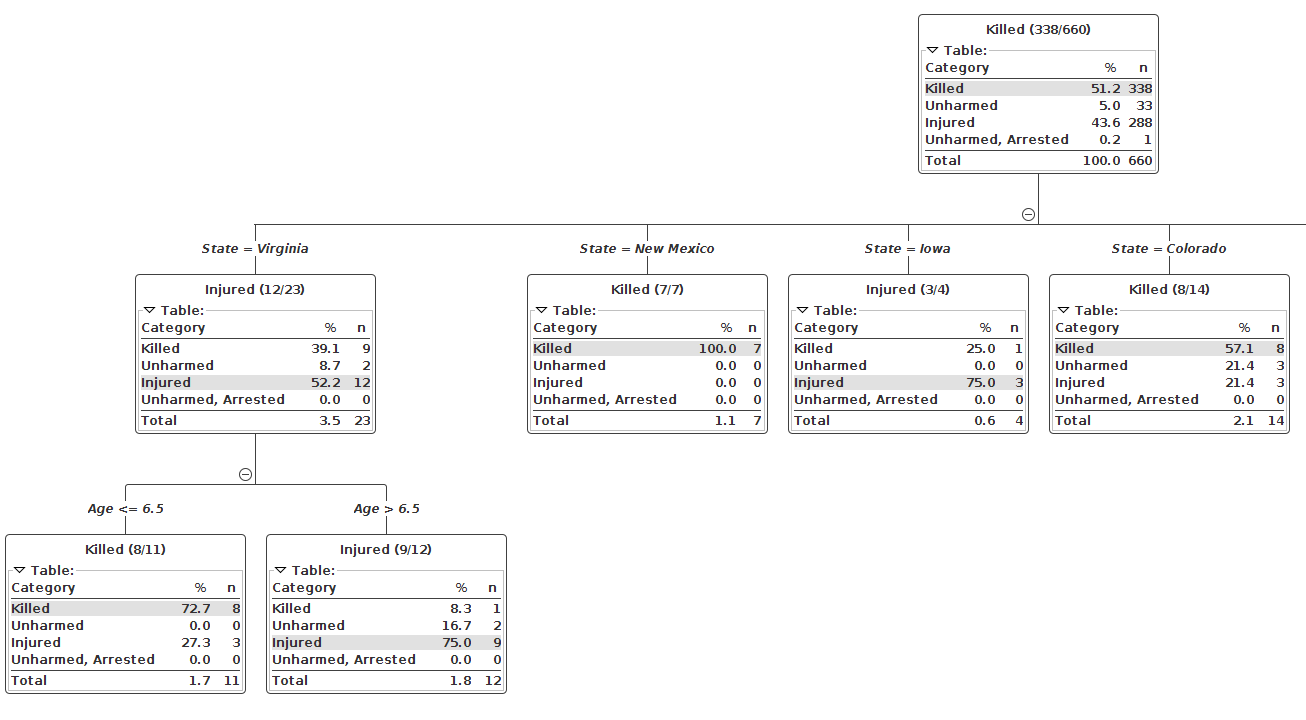
\includegraphics[width=0.9\textwidth]{treeClassifier_splitByState_childrenKI.png}
\caption{Stablo odlu\v civanja po atributu \textit{State}}
\end{figure}

\newpage
\subsubsection{Bajesov algoritam}
Bajesov algoritam radi sa verovatno\' cama i vidimo da se pokazao malo bolje nego stabla odlu\v civanja.
Kori\v s\' cen parametar je podrazumevana verovatno\' ca (0.001) koja nam omogu\' cava malo precizniju klasifikaciju.\break

Preko matrice konfuzije, vidimo da je lo\v sije klasifikovan atribut killed u odnosu na stabla odlu\v civanja, ali je zato atribut injured bolje klasifikovan.
\begin{figure}[H]
\centering
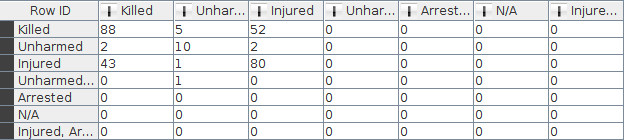
\includegraphics[width=0.9\textwidth]{bayes_confussionMatrix_childrenKI.png}
\caption{Matrica konfuzije za test skup}
\end{figure}

Dobili smo da je preciznost na trening skupu 93\% dok je na test skupu 62.7\%.\\
Iako je preciznost na trening skupu velika, to nam ne garantuje za nove podatke (test skup) da se sna\dj e kako treba jer se previ\v se ugledao na ciljne atribute iz trening skupa.


\subsubsection{K-najbli\v zih suseda}
Za ovaj algoritam smo iskoristili petlju po k, koje predstavlja broj najbli\v zih suseda.\\
$k \in [1,15]$\\
Vidimo da je za ovaj algoritam za sad preciznost najbolja, \v cak 85\% u 6. iteraciji za k=9.

\begin{figure}[H]
\centering
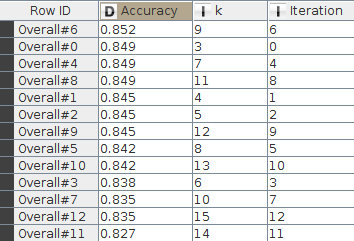
\includegraphics[width=0.4\textwidth]{kNearest_accr_childrenKI.png}
\caption{Preciznost za K najbli\v zih suseda}
\end{figure}

U skladu sa velikom precizno\v s\' cu vidimo na matrici konfuzije da su atributi i killed i injured ovog puta veoma dobro klasifikovani, a takodje i unharmed.

\begin{figure}[H]
\centering
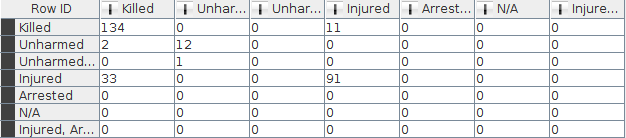
\includegraphics[width=0.9\textwidth]{kNearest_confussionMatrix_childrenKI.png}
\caption{Matrica konfuzije za K najbli\v zih suseda}
\end{figure}

\subsubsection{Neuronska mre\v za}
Primenom ovog algoritma iskoristili smo petlju po broju skrivenih slojeva.\\
$num\_hidden\_layers \in [1,5]$
Ono \v sto mo\v zemo videti da je isto veoma dobra preciznost i na trening i na test skupu, oko 85\%.


\begin{figure}[H]
\centering
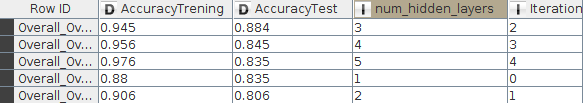
\includegraphics[width=0.6\textwidth]{neuronske_accr_childrenKI.png}
\caption{Preciznost za neuronske mre\v ze}
\end{figure}

Vidimo da je podjednako dobra klasifikacija kao i kod K najbli\v zih suseda.

\begin{figure}[H]
\centering
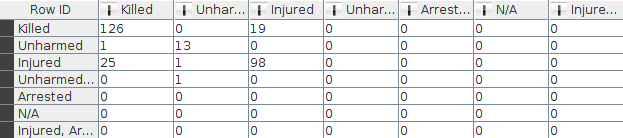
\includegraphics[width=0.9\textwidth]{neuronske_confussionMatrix_childrenKI.png}
\caption{Matrice konfuzije za neuronske mre\v ze}
\end{figure}

\subsubsection{SVM}
SVM klasifikacija je zasnovana na ideji vektorskih prostora, gde \v zelimo na\' ci razdvajaju\' cu hiper-ravan, tako da su svi podaci iz date klase na jednoj strani ravni.\\

Ovaj algoritam je zasnovan na binarnim podacima,
ali iz svih ovih algoritama, videli smo da nam se podaci naj\v ce\v sce klasifikuju u killed ili injured. \\

U parametrima mo\v zemo da biramo razli\v cite kernele, odnosno
\begin{itemize}
\item Polynomial kernel\\
Za power=1, bias=1, gamma=1 preciznost je 0.2\% za trening i 0.4\% za test skup.  
\item HyperTangent\\
Preciznost ista kao i za polinomijalni kernel.
\item RBF\\
Za sigma=0.1 preciznost za trening skup je oko 50\% i 60\% za test skup.  
\end{itemize}
  
Najbolje se pokazao RBF kernel.

\begin{figure}[H]
\centering
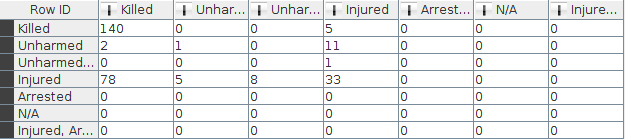
\includegraphics[width=0.9\textwidth]{svm_confussionMatrix_childrenKI.png}
\caption{Matrice konfuzije za SVM koriste\' ci RBF kernel}
\end{figure}


\newpage
\subsection{Predikcija klasifikacijom KNN}
Interesantno bi bilo, koriste\' ci algoritam K-najbli\v zih suseda, izvr\v siti predikciju o statusu osobe na osnovu nekih datih podataka. Ilustrujmo takav primer u Python-u uz kori\v s\' cenje modula \textbf{sklearn}.

\begin{verbatim}
Prilog: knnClassifier.py
\end{verbatim}

Prvo treba u\v citati \v zeljeni csv fajl i izbaciti atribute koji nam nisu od zna\v caja, kao \textit{ID} ili \textit{Name} koji su uvek razli\v citi, a potom i nedostaju\' ce vrednosti:

\begin{lstlisting}
from sklearn.model_selection import train_test_split
from sklearn.neighbors import KNeighborsClassifier
from sklearn.metrics import classification_report, confusion_matrix
import pandas as pd
import numpy as np
from sys import exit, argv

df = pd.read_csv(argv[1])
#izbacujemo neke nevazne atribute
df = df.drop(['ID', 'Name', 'Age Group', 'Incident Date', 'Geolocation', 'Gun Types', 'Guns Stolen'], axis=1)
#izbacujemo instance sa nedostajucim vrednostima
df = df.replace("N/A", np.nan)
df = df.dropna()
#prikaz pocetnih podataka
print(df.head())
\end{lstlisting}


Treba izbaciti i \textit{Status} jer on predstavlja ciljni atribut za koji vr\v simo predikciju. Dalje, sve kategori\v cke podatke predstavljene stringovima treba zameniti jedinstvenim brojem, \v sto se lako mo\v ze ostvariti preko mape  $int \to string$ kao strukture podataka.\footnote{Treba za ciljni atribut napraviti i inverznu mapu da bismo od dobijenog (int) rezultata dobili koja je to (string) kategorija u na\v sem slu\v caju} Pogledajmo na primeru za Status. Za ostale atribute je sli\v cno:

\begin{lstlisting}
final_attr = 'Status'
#izbacujemo Status, njega pogadjamo
X = df.drop([final_attr], axis=1)
#ciljni atribut je Status
y = df[[final_attr]]

#sve menjamo jedinstvenim brojevima
status = df[final_attr].unique()
status_dict = dict(zip(status, range(len(status))))
y = y.replace(status_dict)

#invertovana mapa za status
inv_dict = {v: k for k, v in status_dict.items()}
\end{lstlisting}

\newpage
Sada mo\v zemo podeliti skup na trening (70\%) i test (30\%), pozvati algoritam za klasifikaciju primenom K-najbli\v zih suseda sa pode\v senim parametrima i izvr\v siti predikciju za trening i test skup: 

\begin{lstlisting}
#podela na trening i test
X_train, X_test, y_train, y_test = train_test_split(X, y, test_size = 0.3)

#algoritam k suseda
knn = KNeighborsClassifier(n_neighbors = 15, weights = 'distance')
knn.fit(X_train, y_train.values.ravel())

#prediktovane vrednosti
y_train_predicted = knn.predict(X_train)
y_test_predicted = knn.predict(X_test)
\end{lstlisting}

Sa \verb|sklearn.metrics.classification_report(y_test, y_test_predicted)| vidimo kakva je preziznost, odziv, f1-mera i podr\v ska na test ili trening skupu. Za podatke children\_killed vidimo odli\v cnu preciznost na trening skupu, blizu 100\% i oko 60\% na testu. 

Matrice konfuzije dobijamo pozivom funkcije

\verb|sklearn.metrics.confusion_matrix(y_test, y_test_predicted)|.\break

Sada \' cemo izv\v siti predikciju ona osnovu: \textit{State, City, Guns Involved, Type, Age, Gender} koje nam unosi korisnik, prilagoti ulaz funkciji predict i inverznom mapom ispisati kojoj kategoriji pripada uneta osoba:

\begin{lstlisting}
in_data = []
describe = X.describe()

print("\nUnesi sledece podatke:")
for col in describe.columns:
    print('{:20} min: {:6}, max: {:6}'.format(col, describe[col]['min'], describe[col]['max']))

try:
    in_state = State_dict[input()]
    in_city = City_dict[input()]
    in_guns = int(input())
    in_type = Type_dict[input()]
    in_age =  int(input())
    in_gender = Gender_dict[input()]
except KeyError as e:
    print("Dati podatak nije validan!")
    exit(1)

in_data = [in_state, in_city, in_guns, in_type, in_age, in_gender]
person = np.array(in_data)
person = person.reshape(1, -1)
print("Uneta osoba je: ", inv_dict[knn.predict(person)[0]])
\end{lstlisting}
Pogledajmo jedan primer izlaza ovog programa za neke konkretne unete podatke, kao i pomenute statistike i matrice konfuzije:

\newpage
\begin{verbatim}
report_train: precision    recall  f1-score   support

          0       0.99      1.00      1.00       496
          1       1.00      1.00      1.00        20
          2       0.99      1.00      0.99        92
          3       0.98      0.94      0.96        48
          4       1.00      0.95      0.98        21
          5       1.00      0.83      0.91         6

avg / total       0.99      0.99      0.99       683
report_test:  precision    recall  f1-score   support

          0       0.78      0.97      0.86       205
          1       0.00      0.00      0.00        13
          2       0.73      0.51      0.60        47
          3       0.00      0.00      0.00        20
          4       0.00      0.00      0.00         8
          5       0.00      0.00      0.00         1

avg / total       0.66      0.76      0.70       294
confusion matrix train:
 [[496   0   0   0   0   0]
 [  0  20   0   0   0   0]
 [  0   0  92   0   0   0]
 [  3   0   0  45   0   0]
 [  0   0   1   0  20   0]
 [  0   0   0   1   0   5]]
confusion matrix test:
 [[198   0   4   3   0   0]
 [ 12   0   1   0   0   0]
 [ 19   0  24   1   3   0]
 [ 18   0   2   0   0   0]
 [  5   1   2   0   0   0]
 [  1   0   0   0   0   0]]

Unesi sledece podatke:
State                min:    0.0, max:   44.0
City                 min:    0.0, max:  318.0
Guns Involved        min:    1.0, max:    4.0
Type                 min:    0.0, max:    1.0
Age                  min:    0.0, max:   82.0
Gender               min:    0.0, max:    1.0
> New Jersey
> Stratford
> 1
> Subject-Suspect
> 45
> Male
Uneta osoba je:  Unharmed, Arrested
\end{verbatim}

\newpage
\listoffigures
\listoftables

\end{document}